% ----------------------------------------------------------------
% Article Class (This is a LaTeX2e document)  ********************
% ----------------------------------------------------------------
\documentclass[10pt]{article}
\usepackage[british]{babel}  %% Language
\usepackage[a4paper, margin=1in]{geometry} %% margins
\usepackage{graphicx} % Graphics - allows import of images
\usepackage{float} % Allows for control of float positions
\usepackage[english]{babel}
\usepackage{algorithm}
\usepackage{algorithmic}
\usepackage[noend]{algpseudocode}

\usepackage{float}
\usepackage[bookmarks=true]{hyperref} % 
\usepackage{graphicx}
\usepackage[export]{adjustbox}
\usepackage{wrapfig}
\usepackage{datetime}
\newdate{date}{06}{04}{2022}

%----------------------------------------------------------------

% Title page

%----------------------------------------------------------------
\begin{document}
\title{Configuration Manual}%
%%%%

\author{Srijeet \underline{Gopalan} \\ 20206283 \\ MSc in Cloud Computing}%

\maketitle
% ----------------------------------------------------------------



%----------------------------------------------------------------

% Table of contents

%----------------------------------------------------------------
\tableofcontents
\thispagestyle{empty}
\cleardoublepage
\setcounter{page}{1}

%----------------------------------------------------------------

% Main Headings Section

%----------------------------------------------------------------


\section{Introduction} 
This manual aims to educate users on all of the tools, programs, and procedures needed to implement the project. To help the user understand the configuration required to complete a particular tasks, it comprises of text and visual elements (drawings, screenshots, infographics, etc.).

\section{Hardware Requirements}
\subsection{System Requirement}

\begin{table}[H]
\begin{tabular}{|l|l|}
\hline
\textbf{Operating System} & Microsoft Windows 10 Home \\ \hline
\textbf{Processor} & Intel Core i7-9750H @ 2.60GHz \\ \hline
\textbf{Installed Ram} & 4 GB \\ \hline
\textbf{Storage} & 1 TB HDD \\ \hline
\end{tabular}
\end{table}
\subsection{Raspberry Pi Requirement}

\begin{table}[]
\begin{tabular}{|l|l|}
\hline
\textbf{Operating System} & Raspios\_oldstable\_armhf-2021-12-02 \\ \hline
\textbf{Processor} & Quad Core Cortex A27 ARM V8 64bit @ 1.5GHz \\ \hline
\textbf{Installed Ram} & 4 GB \\ \hline
\textbf{Storage} & 32 GB SD Card \\ \hline
\end{tabular}
\end{table}

\section{Software Requirements}
\subsection{Visual Studio 2019 Community Edition}
\begin{itemize}
    \item Download Visual Studio from https://visualstudio.microsoft.com/downloads/ \cite{2}.
\item Select Visual Studio Community Edition.
\item Install vs community.exe, the Visual Studio installer.
\item Accept the Microsoft Privacy Statement as well as the Microsoft License Terms. Select Continue.
\item Follow the installation instructions displayed on the screen.
\item Once Visual Studio has been installed, click the Launch button to begin building with Visual Studio.
\item Fig \ref{fig:vs} depicts the Visual studio IDE.
\end{itemize}
\begin{figure}[H]
    \begin{center}
        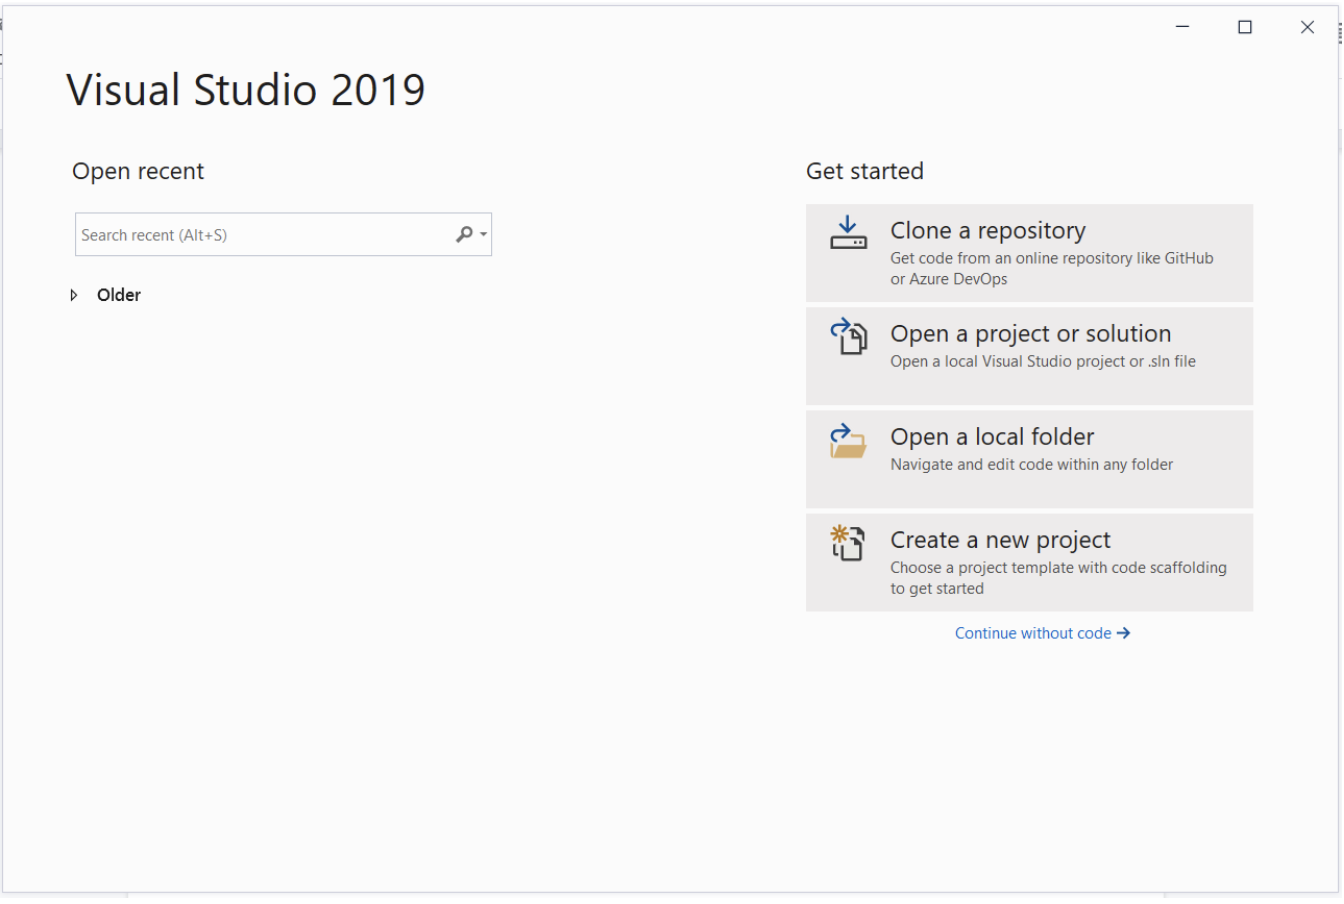
\includegraphics[width=0.7\linewidth, frame]{CA2-template/CM4.png}
       \caption{Visual Studio 2019 Community Edition \label{fig:vs}}
    \end{center}
\end{figure}

\subsection{Visual Studio Code}
\begin{itemize}
    \item Download the executable document from https://code.visualstudio.com/download \cite{3}.
\item Click the ch Download on windows version
\item Accept the agreement after opening the downloaded file, then click Next.
\item Follow the installation instructions displayed on the screen.
\item To finish setup, click Finish. To start VS Code right away, check the box.
\item Fig \ref{fig:vsc} depicts the VS Code IDE.
\end{itemize}
\begin{figure}[H]
    \begin{center}
        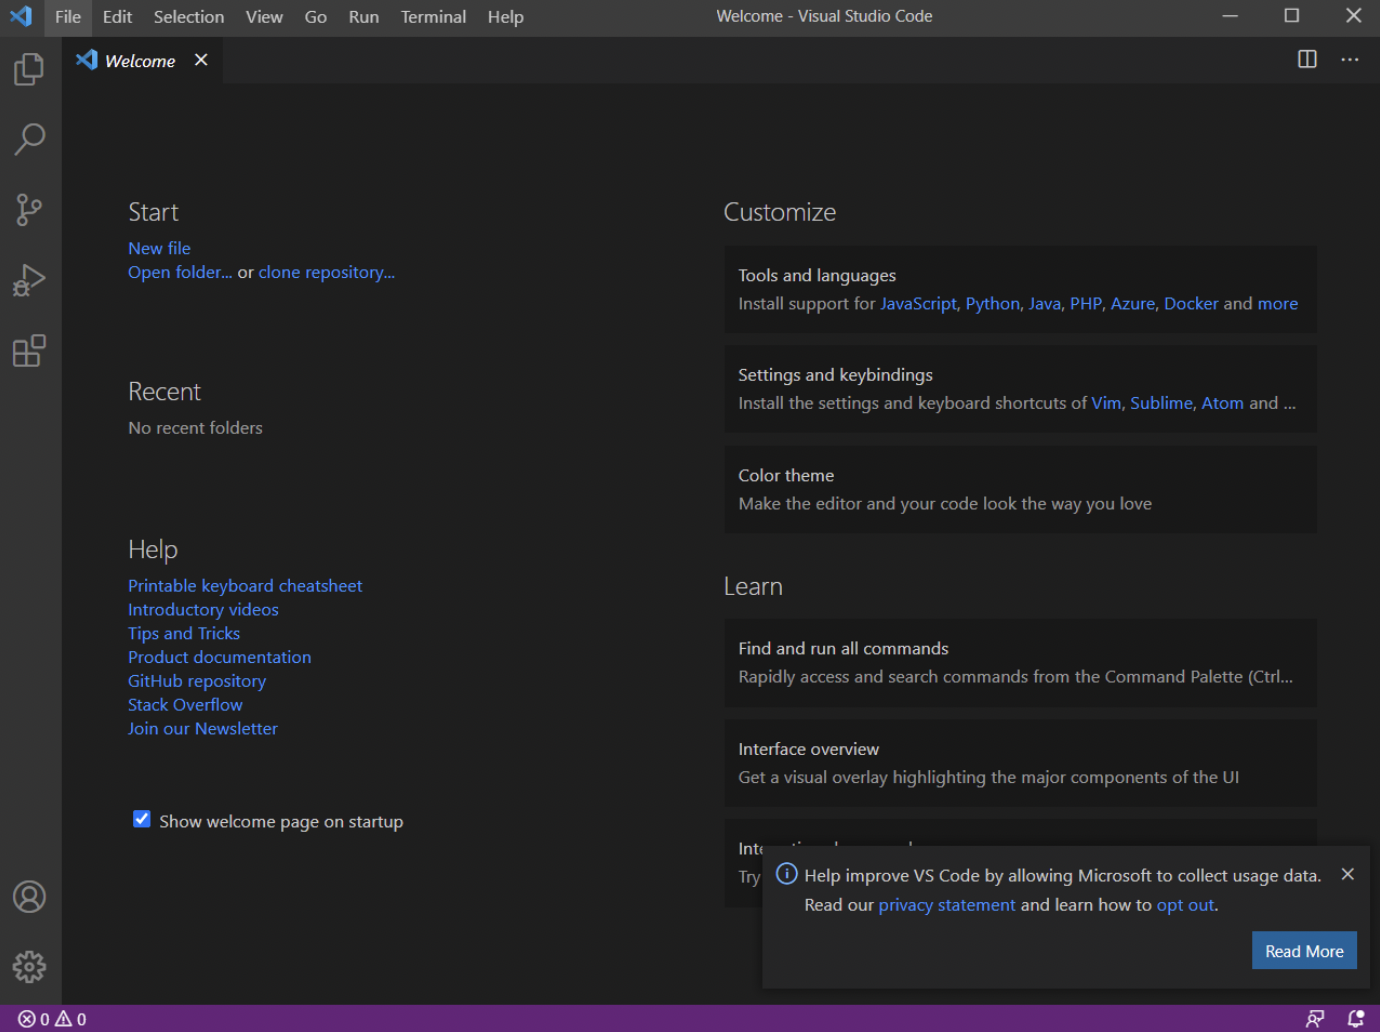
\includegraphics[width=0.7\linewidth, frame]{CA2-template/CM3.png}
       \caption{VS Code \label{fig:vsc}}
    \end{center}
\end{figure}

\subsection{Python 3.6}
\begin{itemize}
    \item Open the Python website in the browser and go to the Downloads for Windows section \cite{4}.
\item Look for Python 3.6.
\item To get the Windows x86-64 executable installer, click on the appropriate link.
\item Once downloaded, launch the Python Installer.
\item Check the box next to "Add Python 3.6 to PATH" and then click "Install now."
\item Go to the location where Python was set up on the computer.
\item Open Python.exe.
\item The result should like Fig \ref{fig:py}
\begin{figure}[H]
    \begin{center}
        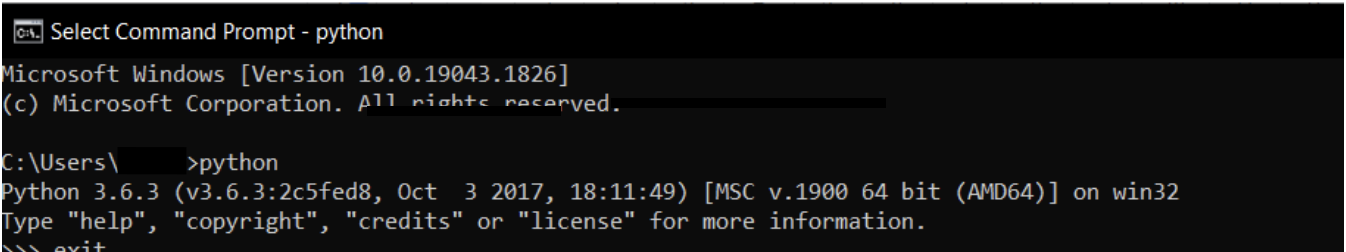
\includegraphics[width=0.7\linewidth, frame]{CA2-template/CM6.png}
       \caption{Python 3.6 \label{fig:py}}
    \end{center}
\end{figure}

\item By typing pip -V in the console, confirm that Pip was installed. If the installation was successful, the output from Fig.\ref{fig:pip} should appear.
\begin{figure}[H]
    \begin{center}
        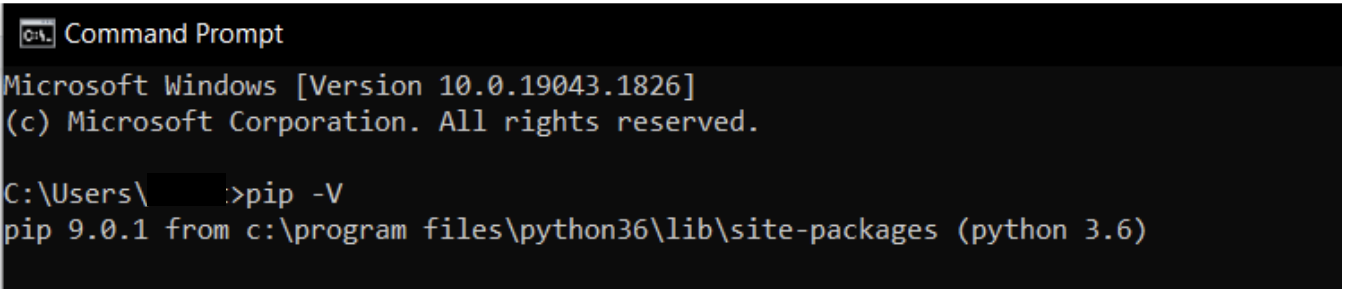
\includegraphics[width=0.7\linewidth, frame]{CA2-template/CM5.png}
       \caption{PIP \label{fig:pip}}
    \end{center}
\end{figure}

\end{itemize}

\subsection{Eclipse IDE}
\begin{itemize}
    \item Eclipse Installer can be downloaded through www.eclipse.org/downloads \cite{5}.
\item Launch the Eclipse Installer program.
\item To install, choose and click the "Eclipse IDE for Java Developers" package.
\item Choose the 'Install' option to start the installation, and then specify the destination installation folder.
\item When the installation is finished, open Eclipse (Fig \ref{fig:eclipse}). 
\begin{figure}[H]
    \begin{center}
        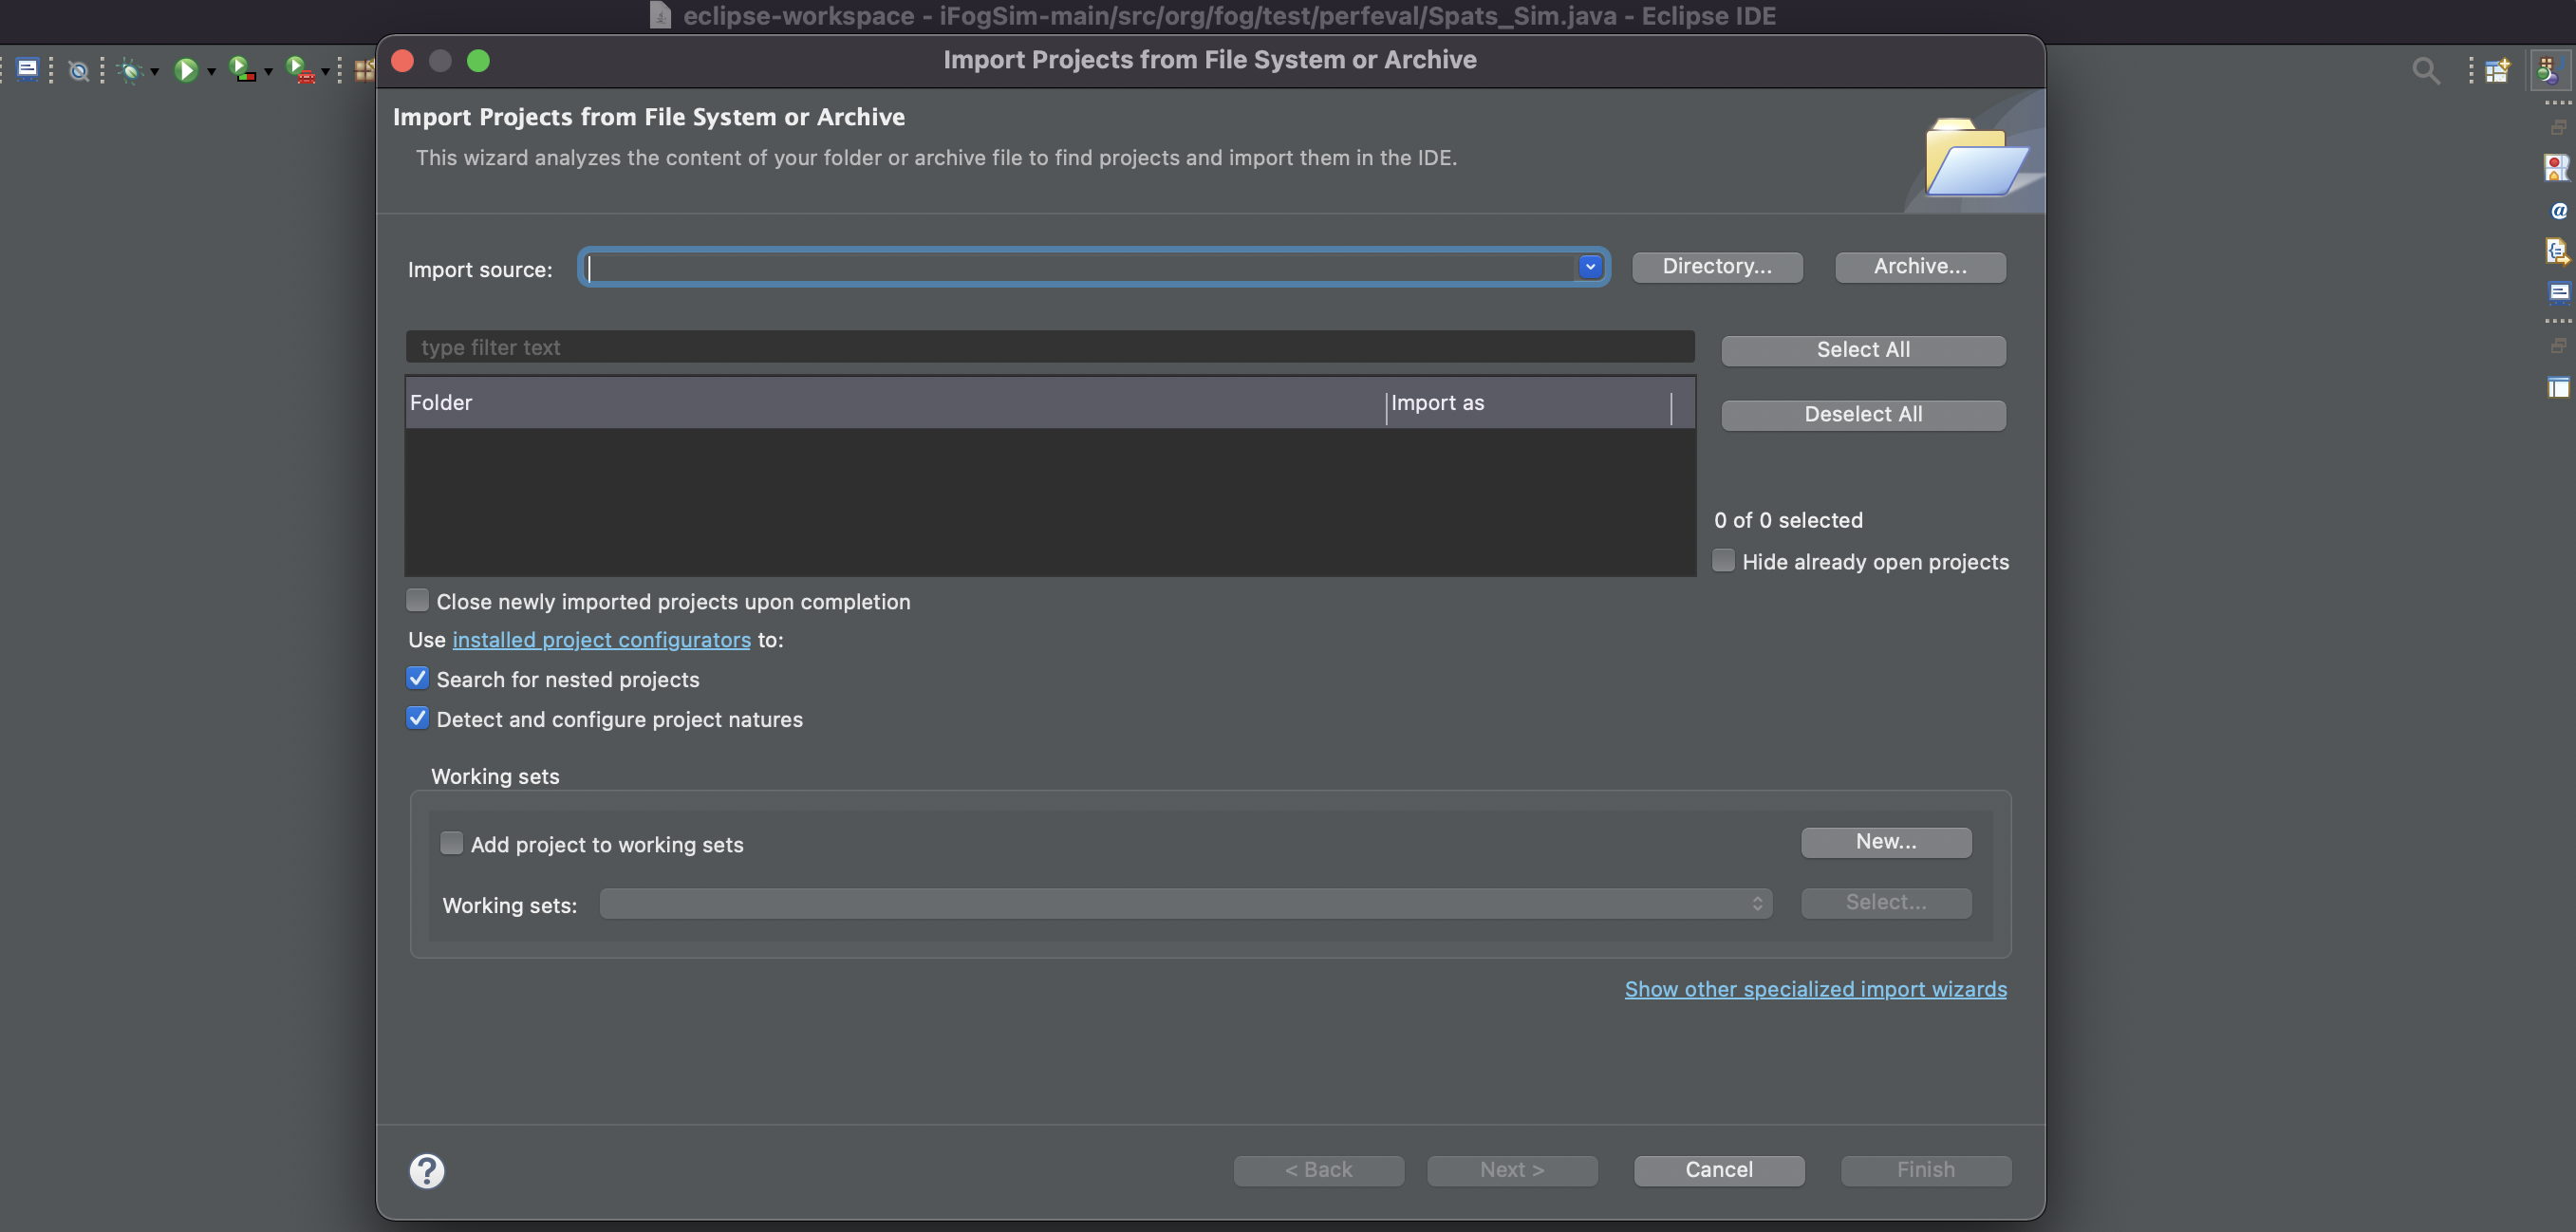
\includegraphics[width=0.7\linewidth, frame]{CA2-template/CM7.png}
       \caption{Eclipse IDE \label{fig:eclipse}}
    \end{center}
\end{figure}
\end{itemize}

\subsection{IFogSim}
\begin{itemize}
    \item Launch Eclipse IDE.
\item Build a Java project.
\item Initialize a blank Git repository within the project directory using the following command:
\newline
init git
\item As the origin remote, add the iFogSim2 Git repository:
\newline git remote add origin https://github.com/Cloudslab/iFogSim \cite{6}
\item Use git pull to download the repository's contents to the local computer:
\newline git pull main origin
\item Add JARS to project.
\item Fig \ref{fig:ifog} shows the IFogSim project contents
\begin{figure}[H]
    \begin{center}
        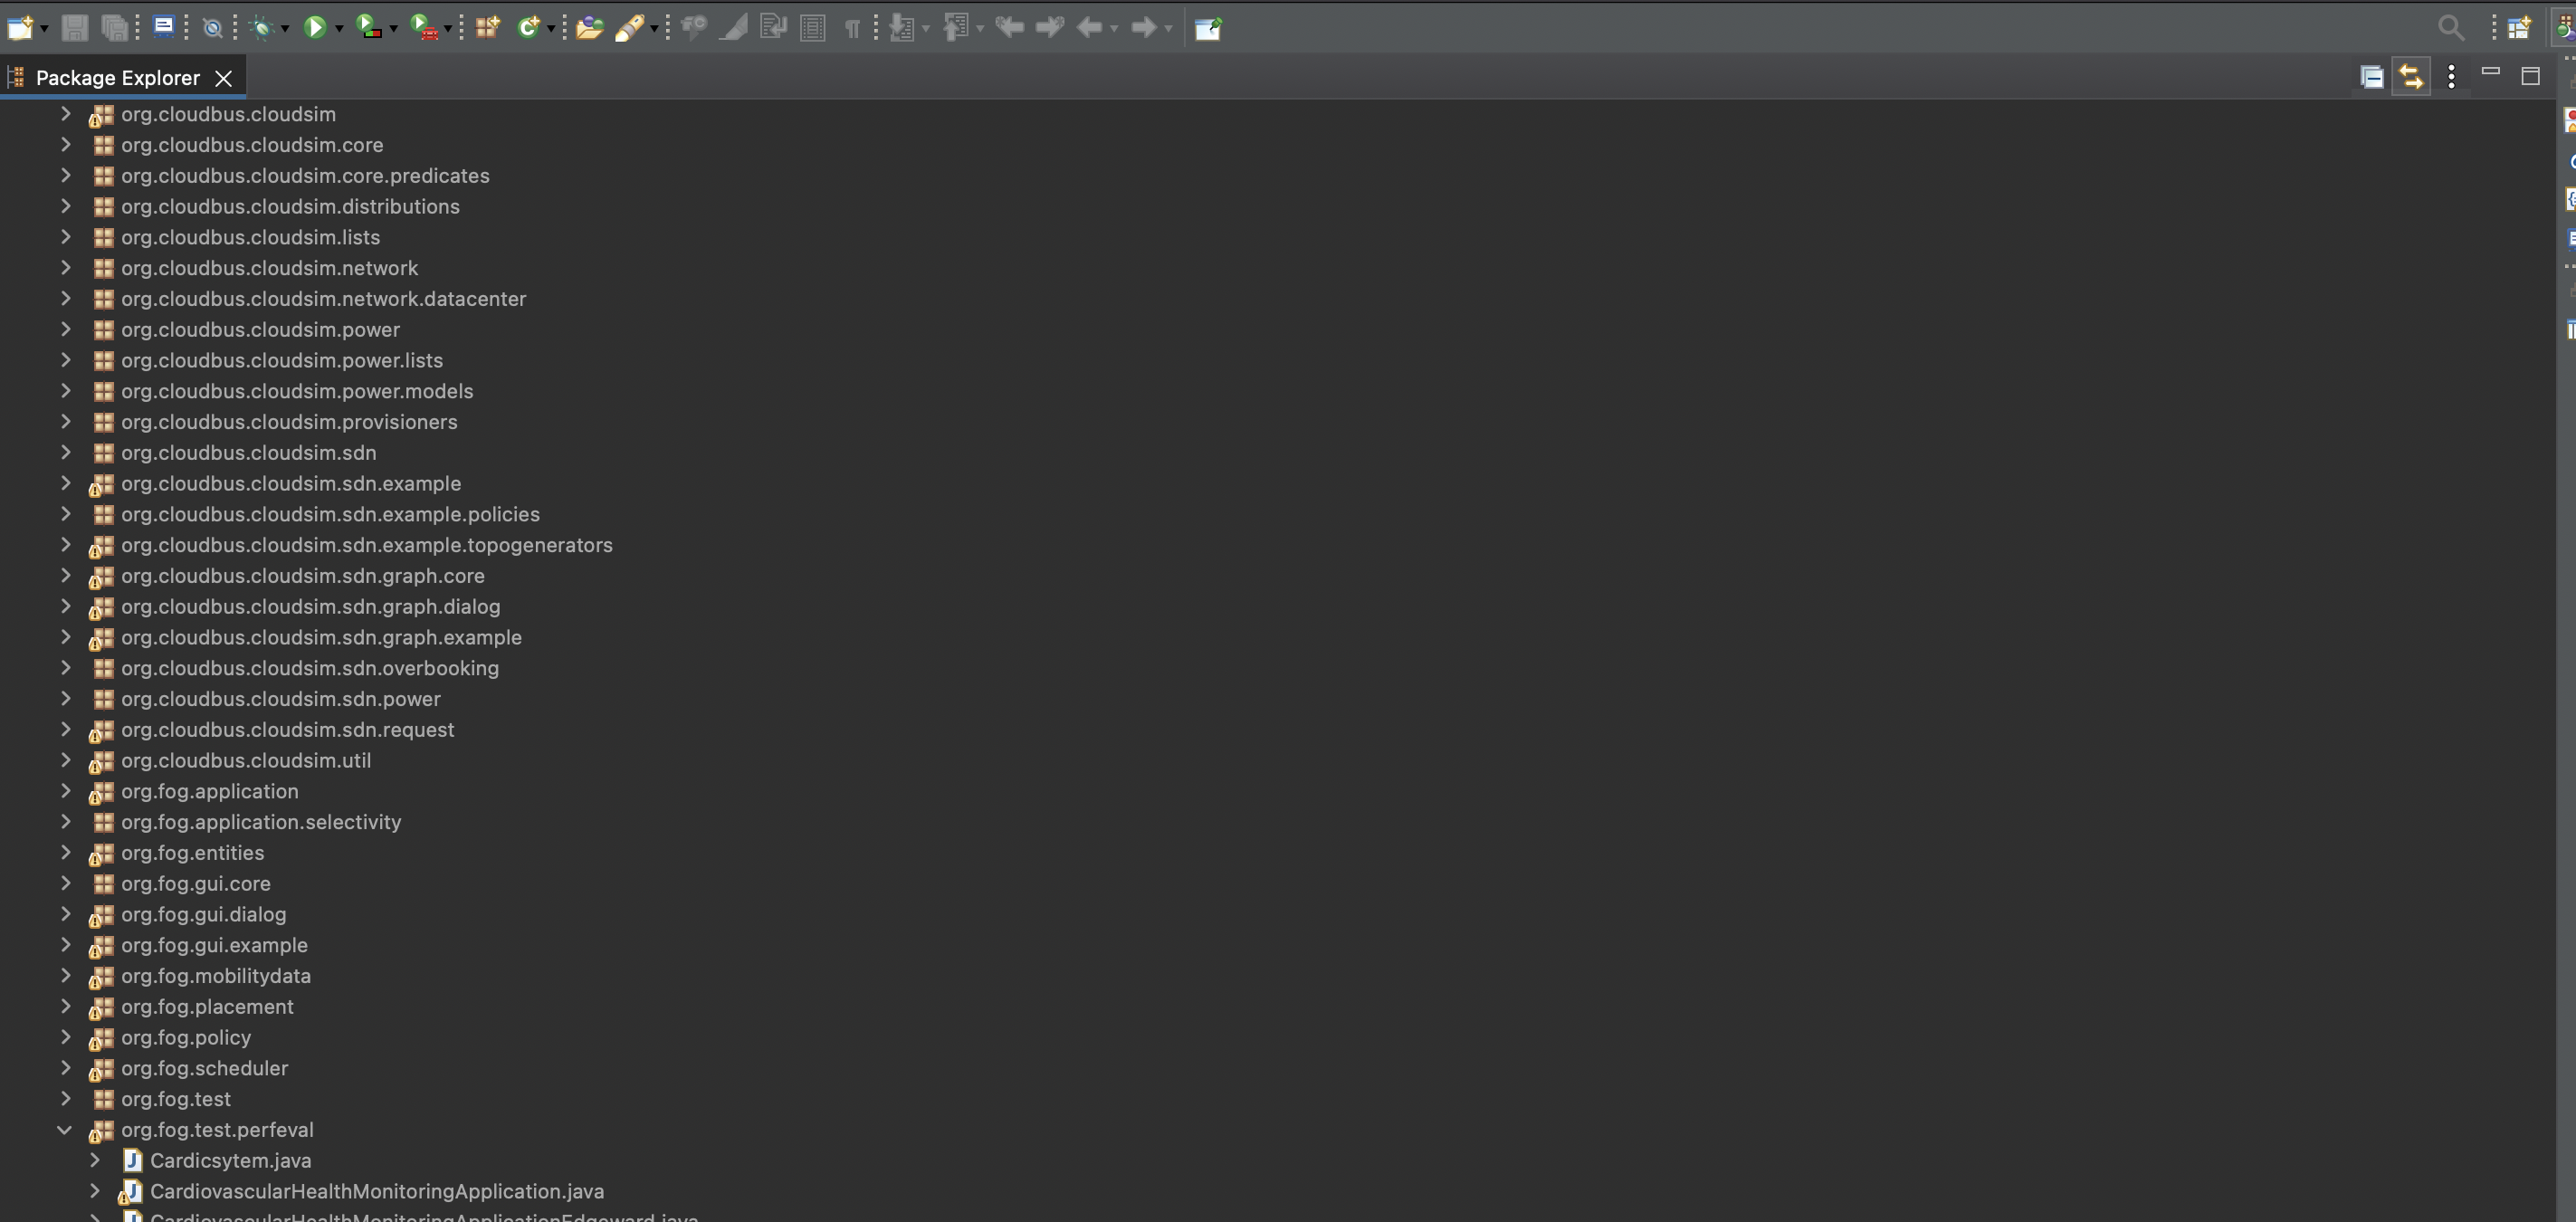
\includegraphics[width=0.7\linewidth, frame]{CA2-template/CM8.png}
       \caption{IFogSim \label{fig:ifog}}
    \end{center}
\end{figure}
\end{itemize}

\section{Implementation}

\subsection{SPATS Web Application}
The SPATS web application is built using ASP.NET with C# and SQL for backend database.
\subsubsection{Run in local server}
\begin{itemize}
    \item Launch Visual Studio 2019 IDE and select "Continue without code" option
    \begin{figure}[H]
    \begin{center}
        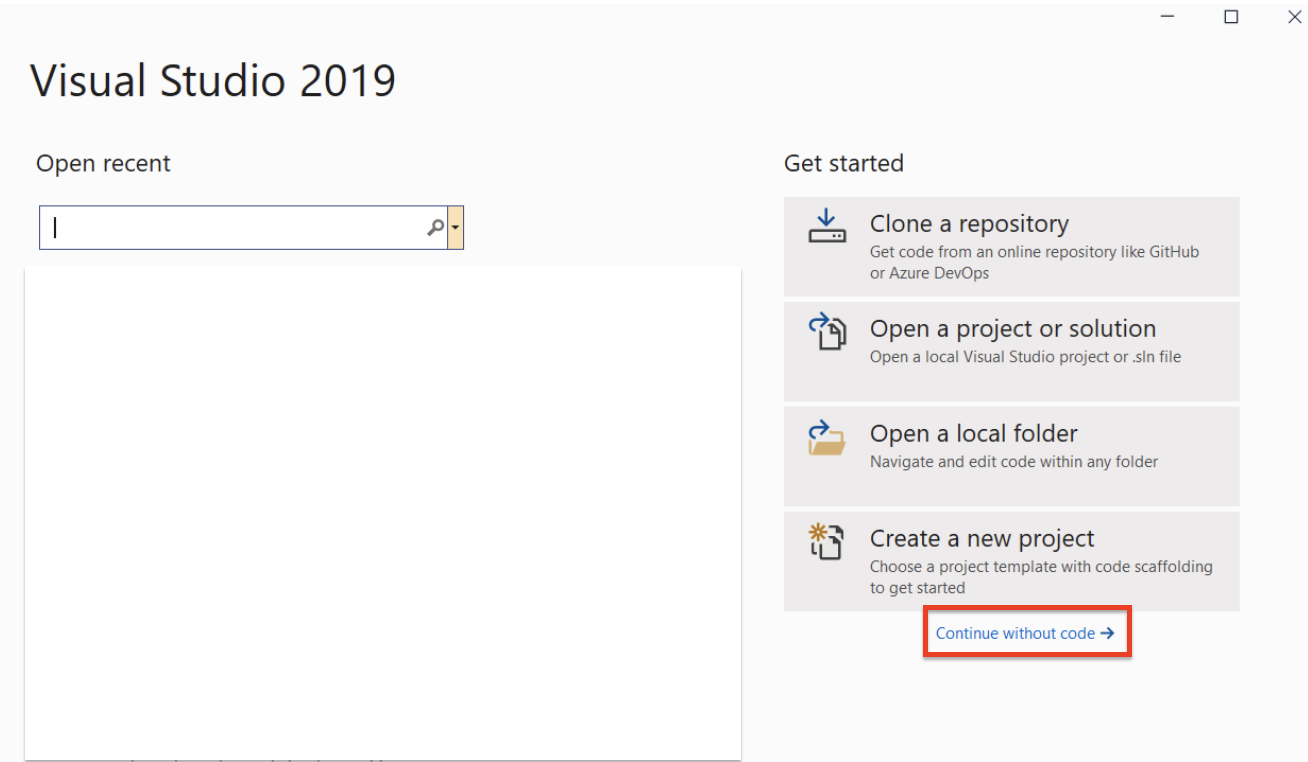
\includegraphics[width=0.7\linewidth, frame]{CA2-template/CM9.png}
       \caption{Visual Studio Start Page \label{fig:1}}
    \end{center}
\end{figure}

\item Goto File menu and select "Website" by clicking on "Open" 
\begin{figure}[H]
    \begin{center}
        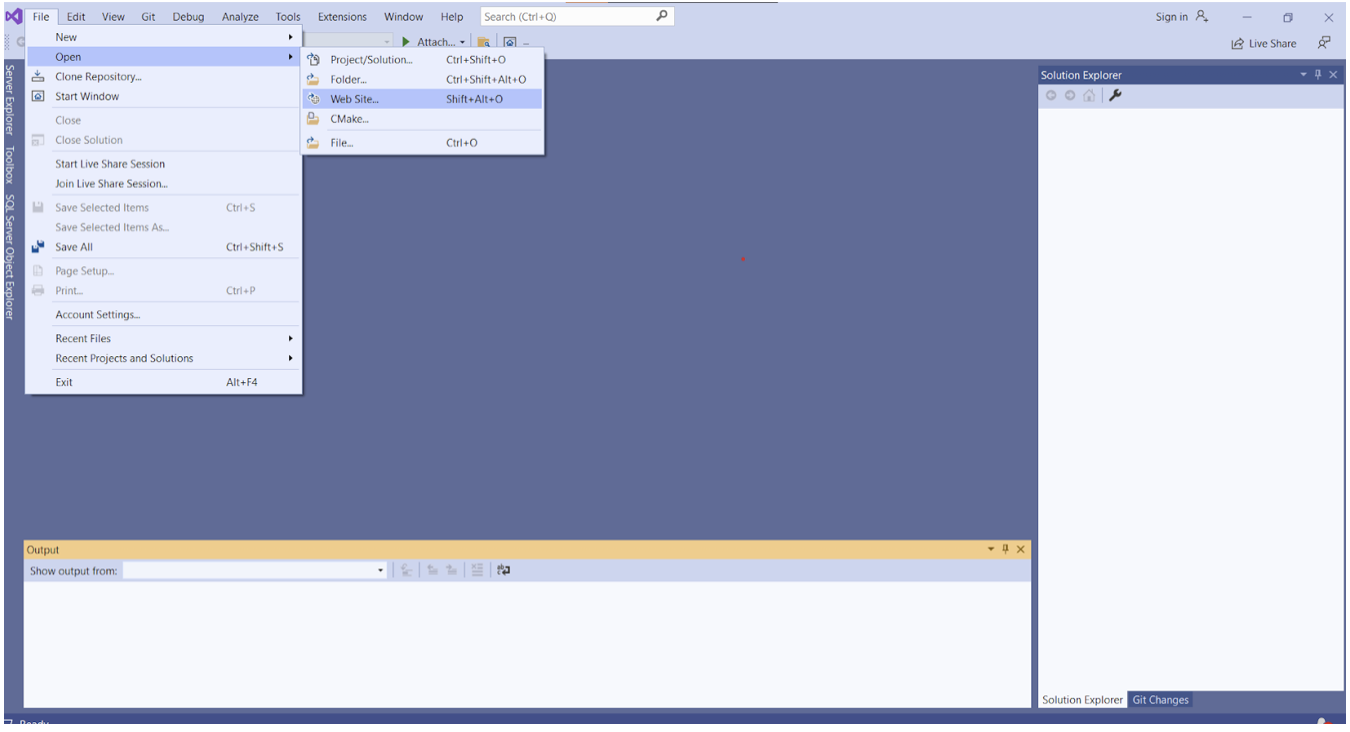
\includegraphics[width=0.7\linewidth, frame]{CA2-template/CM10.png}
       \caption{File Menu \label{fig:2}}
    \end{center}
\end{figure}

\item From the Open dialouge box, navigate to the application folder and click Open
\begin{figure}[H]
    \begin{center}
        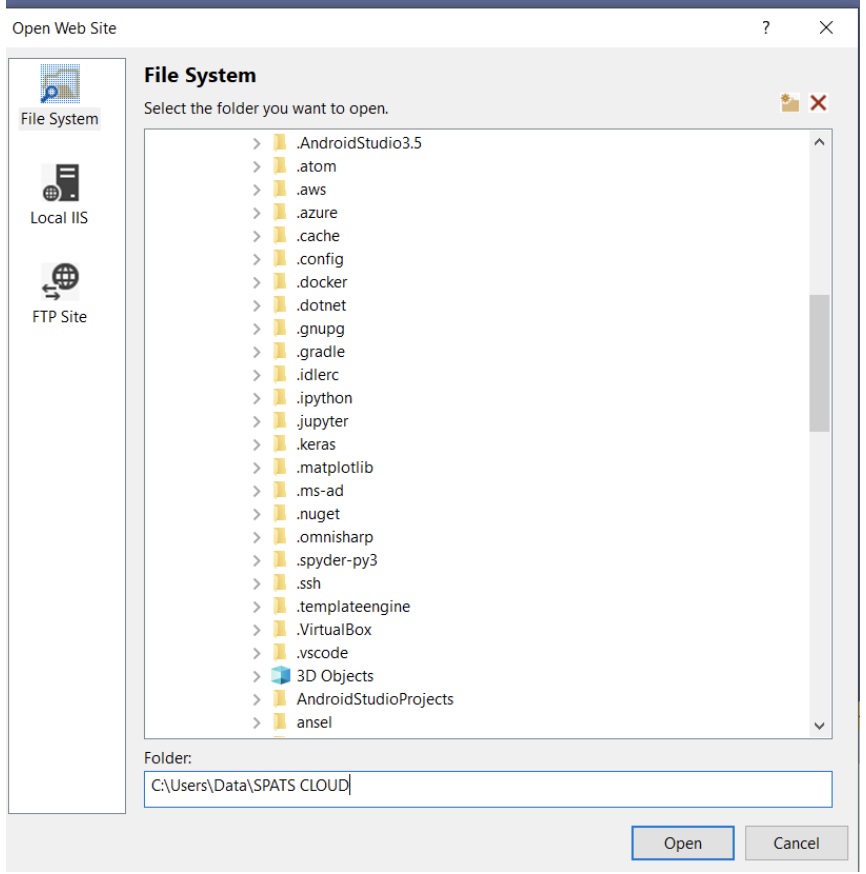
\includegraphics[width=0.7\linewidth, frame]{CA2-template/CM11.png}
       \caption{Open \label{fig:3}}
    \end{center}
\end{figure}

\item From "SQL server Object Explorer", right click on database and select "Add new database" and name it "SPATS CLOUD\_DB 
\begin{figure}[H]
    \begin{center}
        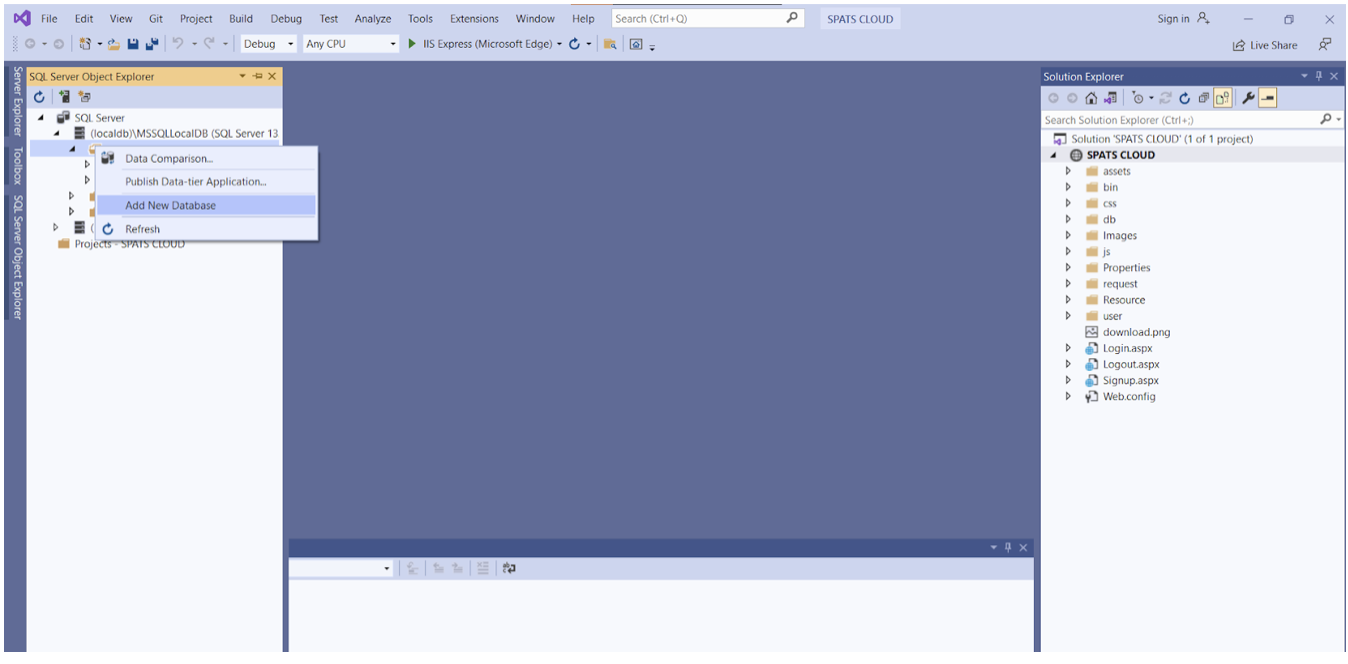
\includegraphics[width=0.7\linewidth, frame]{CA2-template/CM12.png}
       \caption{SQL Server Explorer \label{fig:4}}
    \end{center}
\end{figure}

\item Right Click on the created database and select "New Query"
\begin{figure}[H]
    \begin{center}
        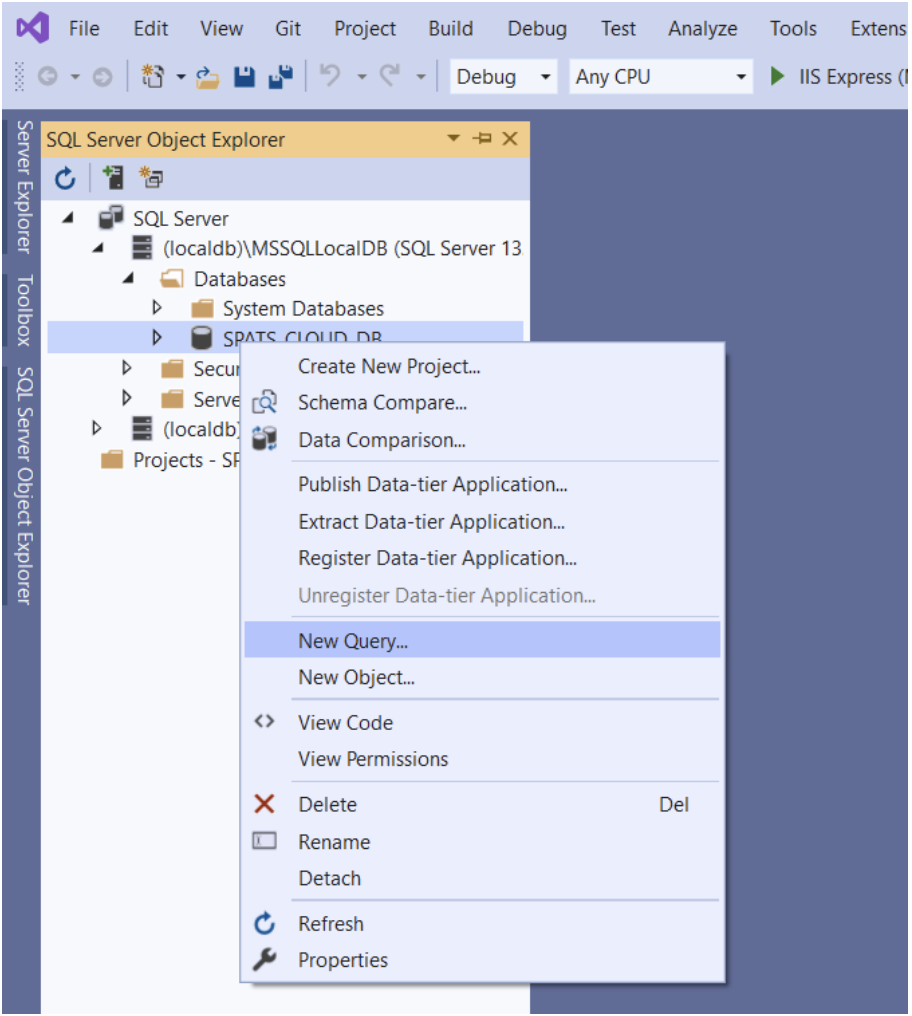
\includegraphics[width=0.7\linewidth, frame]{CA2-template/CM13.png}
       \caption{New Query \label{fig:5}}
    \end{center}
\end{figure}

\item Write the query to create two tables one for user registration and other one for user transaction. Run the query by clicking on the Play button on the top left corner of the window pane.
\begin{figure}[H]
    \begin{center}
        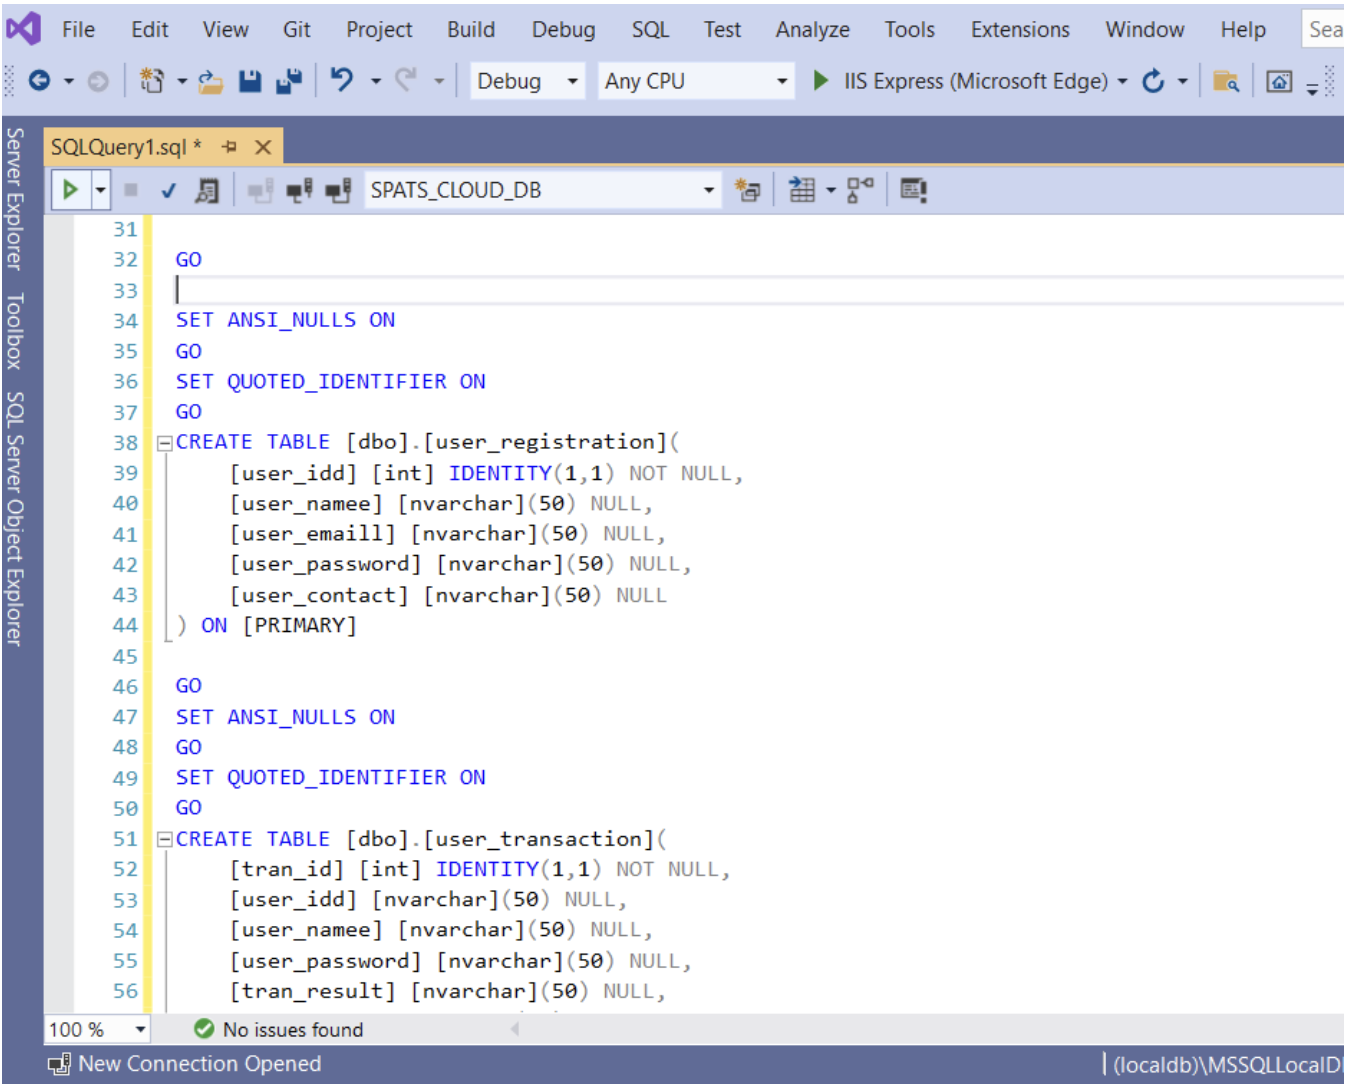
\includegraphics[width=0.7\linewidth, frame]{CA2-template/CM14.png}
       \caption{Run Query \label{fig:6}}
    \end{center}
\end{figure}

\item Open web.config file and make changes in the connectionString as per the name of the database given in the previous step. 
\begin{figure}[H]
    \begin{center}
        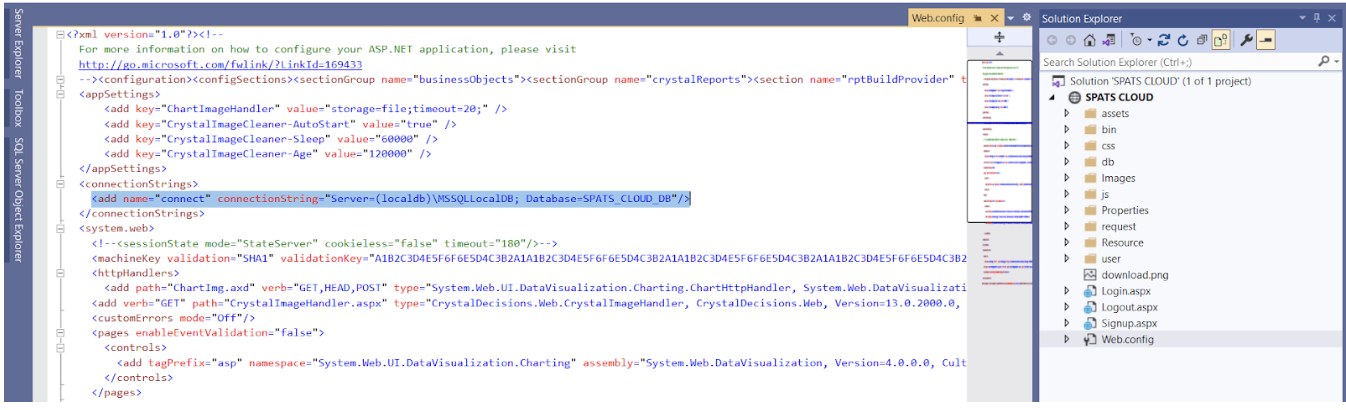
\includegraphics[width=0.7\linewidth, frame]{CA2-template/CM15.png}
       \caption{Connection String \label{fig:7}}
    \end{center}
\end{figure}

\item Set Login.aspx as the start page
\begin{figure}[H]
    \begin{center}
        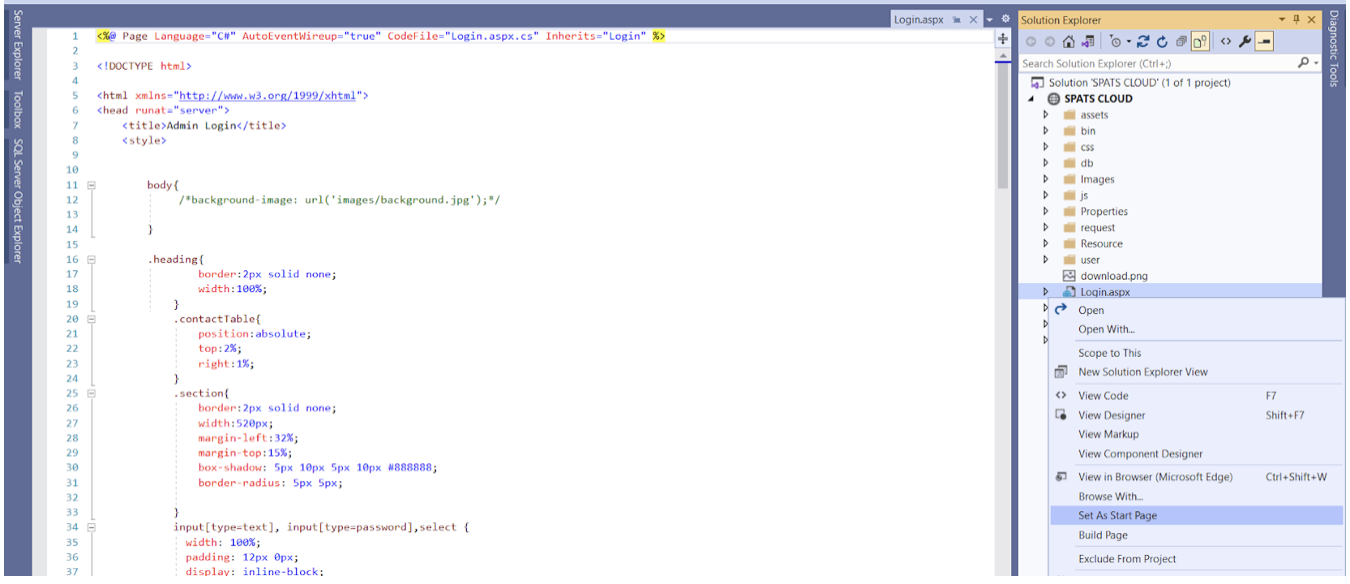
\includegraphics[width=0.7\linewidth, frame]{CA2-template/CM16.png}
       \caption{Set Start Page \label{fig:8}}
    \end{center}
\end{figure}

\item Run the application by clicking on the play button and selecting "IIS Express". The application will open in the browser window as shown in Fig \ref{fig:9}
\begin{figure}[H]
    \begin{center}
        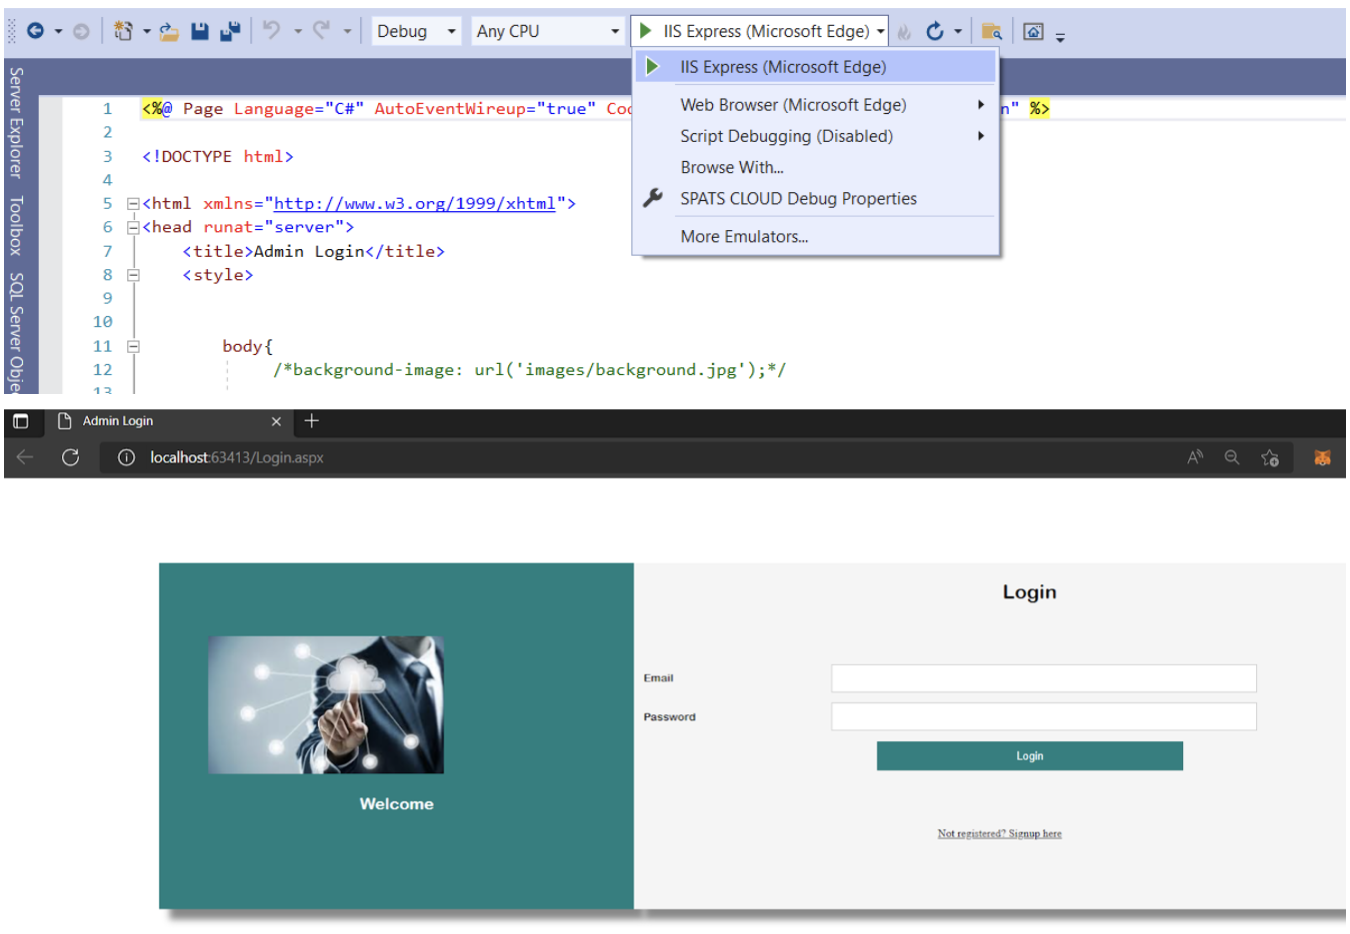
\includegraphics[width=0.7\linewidth, frame]{CA2-template/CM17.png}
       \caption{Run Application \label{fig:9}}
    \end{center}
\end{figure}

\end{itemize}

\subsubsection{Run on Azure VM}
SPATS web application is hosted on Azure Fig \ref{fig:10}. It can be accessed through the below mentioned URL:
\newline https://spats1.azurewebsites.net
\begin{figure}[H]
    \begin{center}
        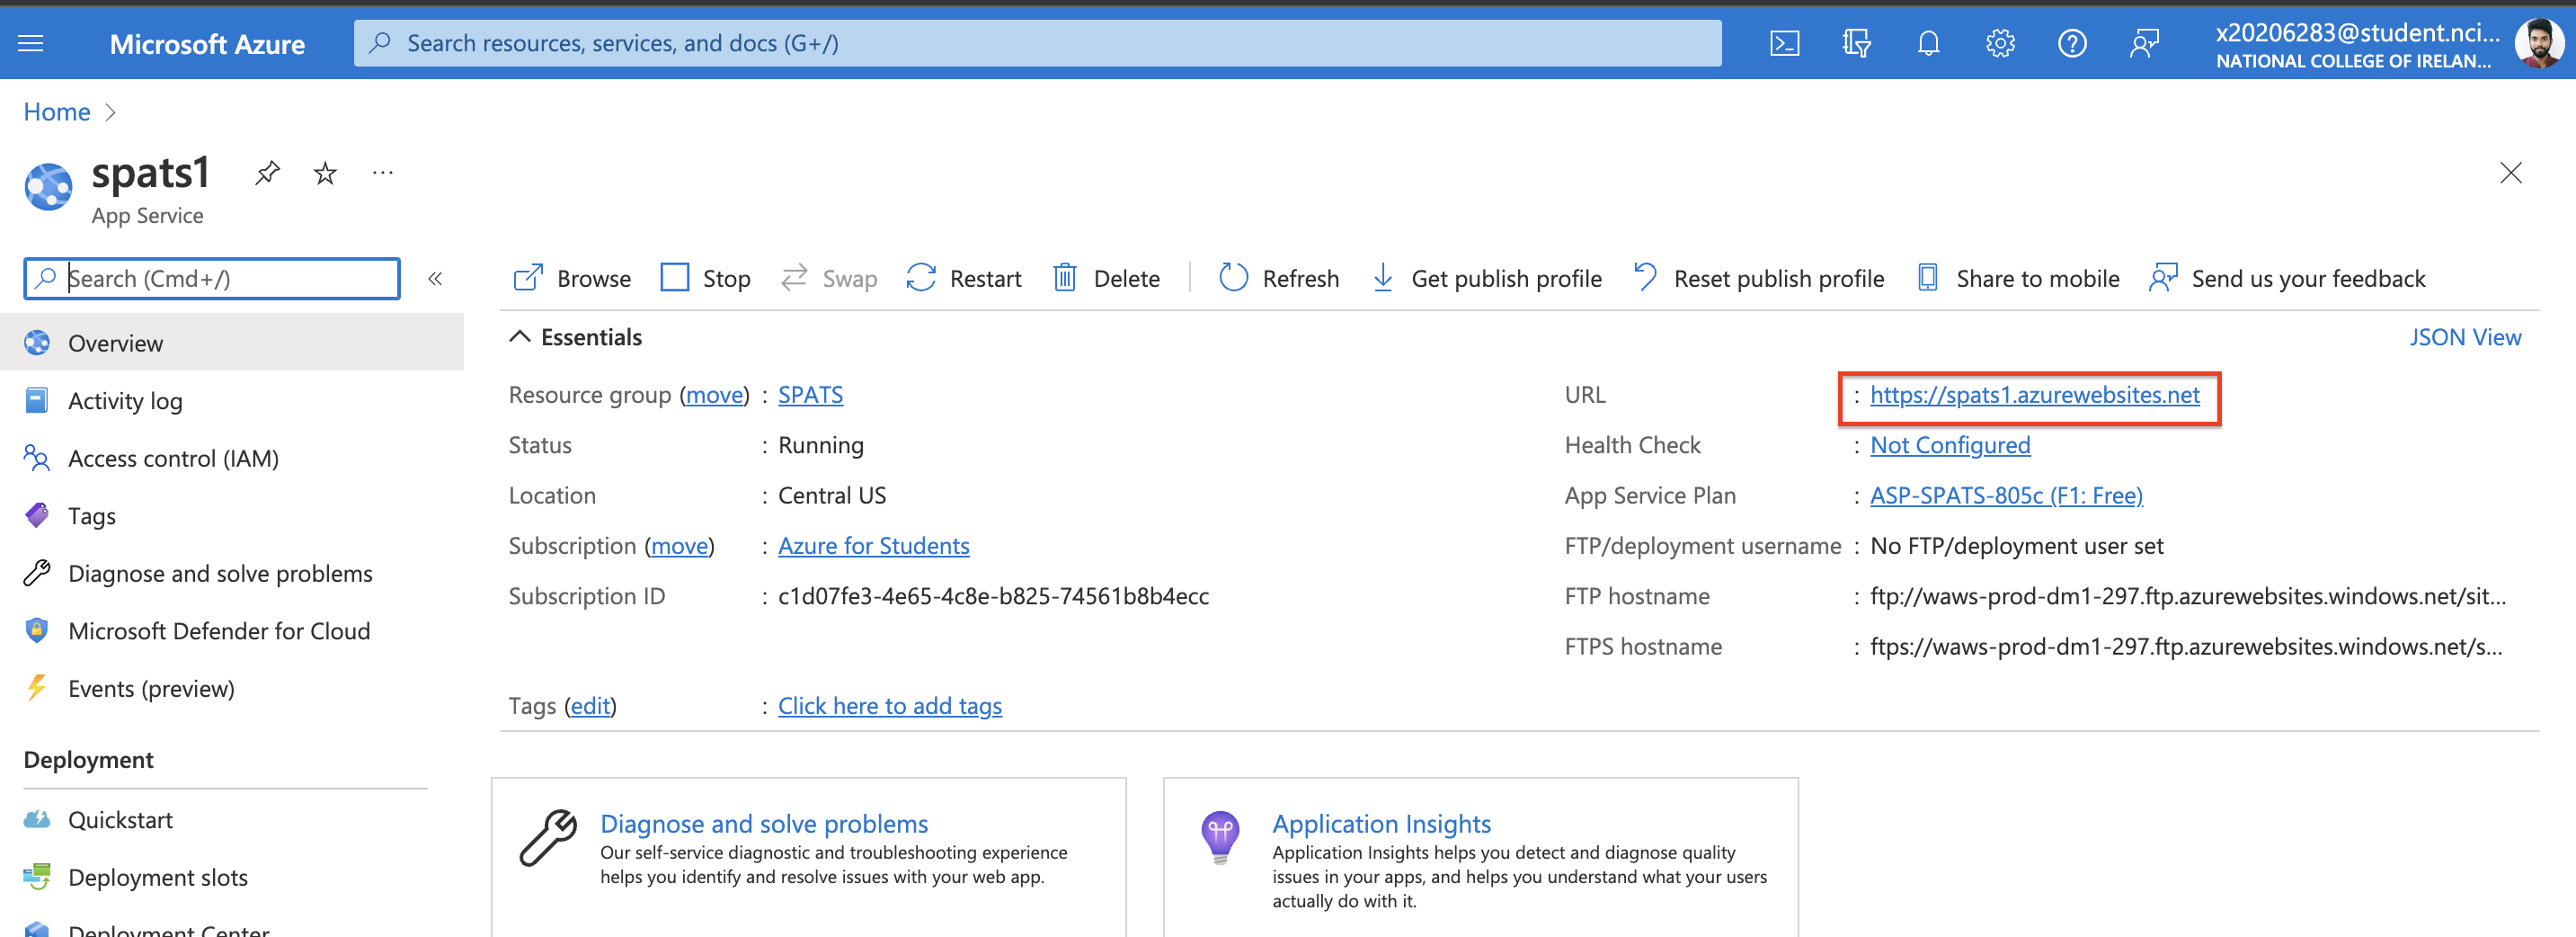
\includegraphics[width=0.7\linewidth, frame]{CA2-template/CM18.png}
       \caption{SPATS on Azure \label{fig:10}}
    \end{center}
\end{figure}

\subsection{SPATS Gateway Application}
This application is built using Python Flask language and Pandas or rather Scikit-learn machine learning libraries. VS Code is used to develop this application.

\subsubsection{Installing the Libraries}
Run Command Prompt and install the following libraries.
\begin{itemize}
    \item pip install pandas
\begin{figure}[H]
    \begin{center}
        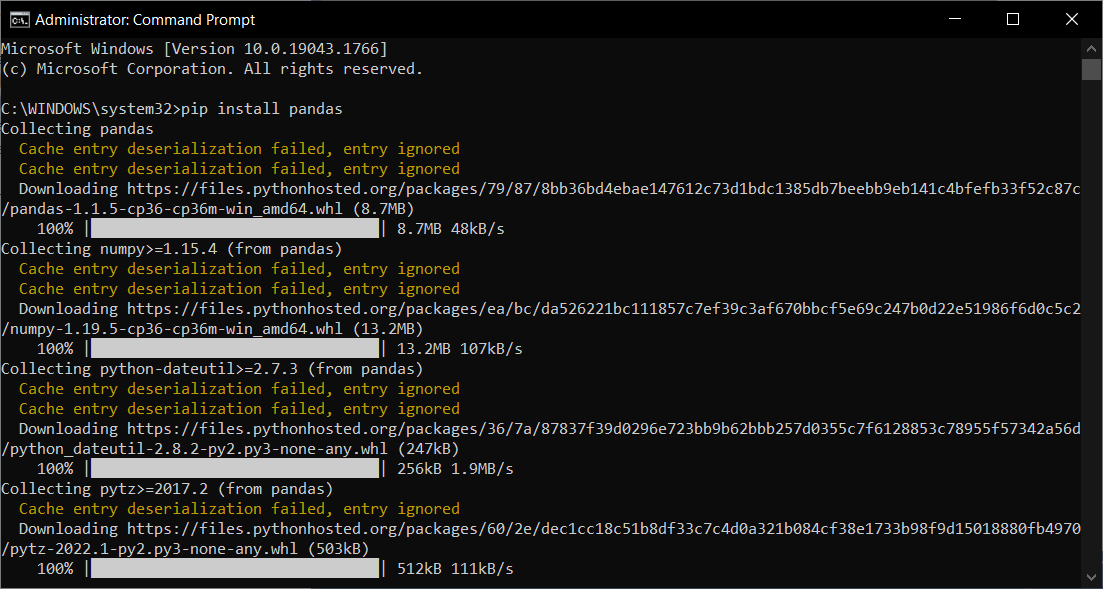
\includegraphics[width=0.7\linewidth, frame]{CA2-template/CM19.png}
       \caption{pandas \label{fig:11}}
    \end{center}
\end{figure}

\item pip install sklearn
\begin{figure}[H]
    \begin{center}
        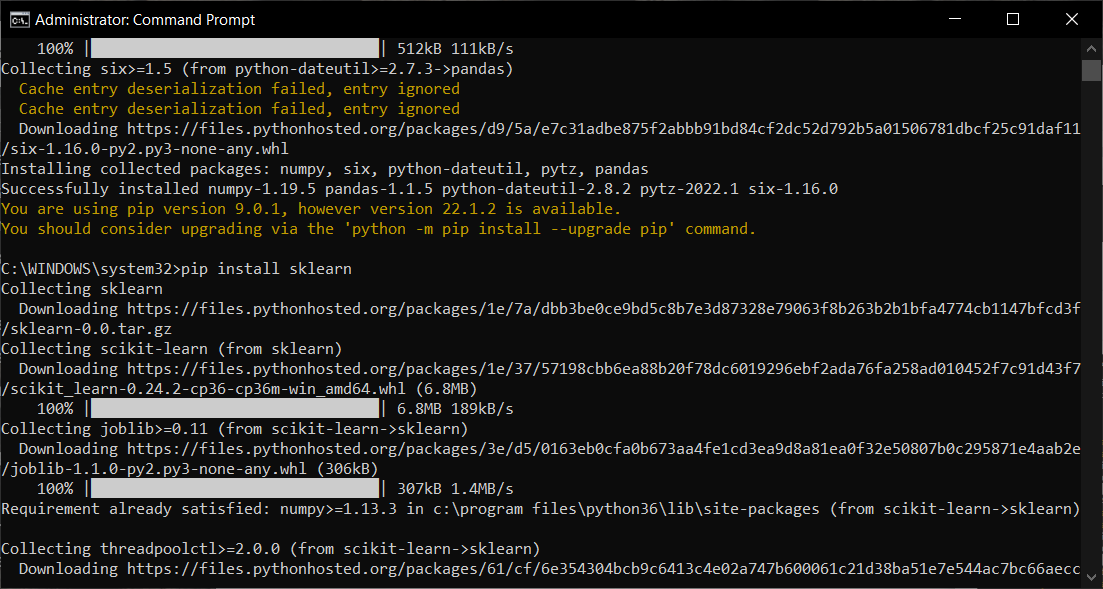
\includegraphics[width=0.7\linewidth, frame]{CA2-template/CM20.png}
       \caption{sklearn \label{fig:12}}
    \end{center}
\end{figure}

\item pip install scikit-learn==0.22.2.post1
\begin{figure}[H]
    \begin{center}
        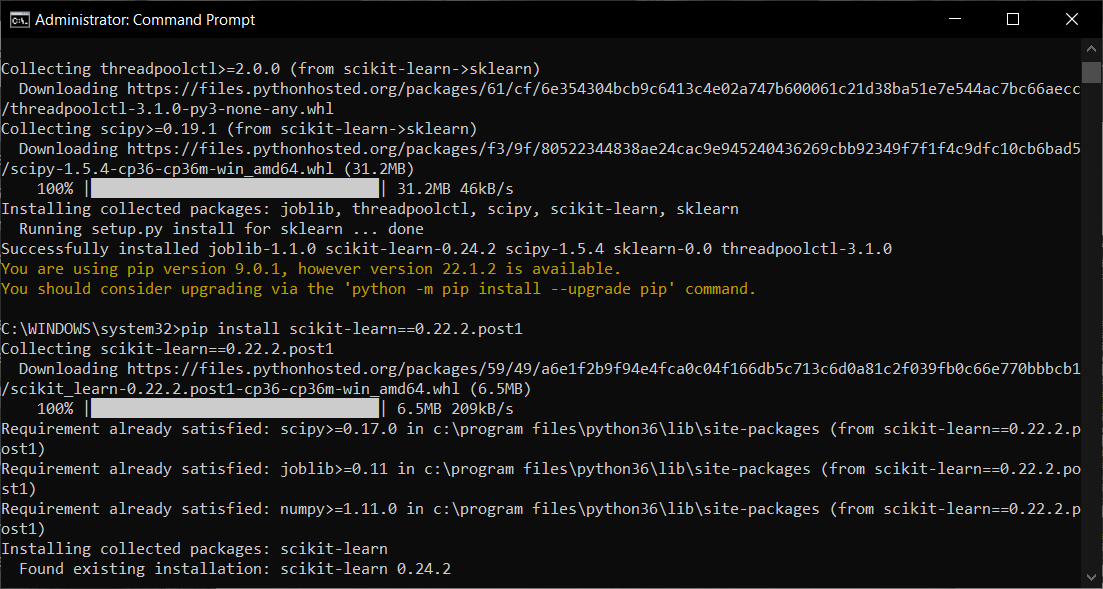
\includegraphics[width=0.7\linewidth, frame]{CA2-template/CM21.png}
       \caption{scikit \label{fig:13}}
    \end{center}
\end{figure}

\item pip install yellowbrick==0.9.1
\begin{figure}[H]
    \begin{center}
        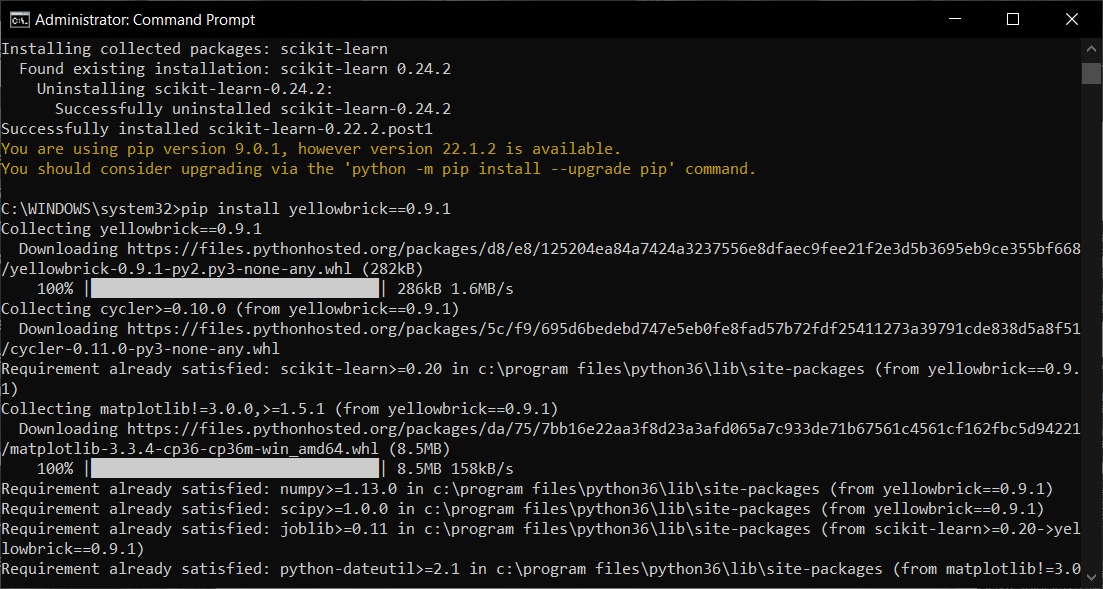
\includegraphics[width=0.7\linewidth, frame]{CA2-template/CM22.png}
       \caption{yellobrick \label{fig:14}}
    \end{center}
\end{figure}

\item pip install seaborn==0.9.0
\begin{figure}[H]
    \begin{center}
        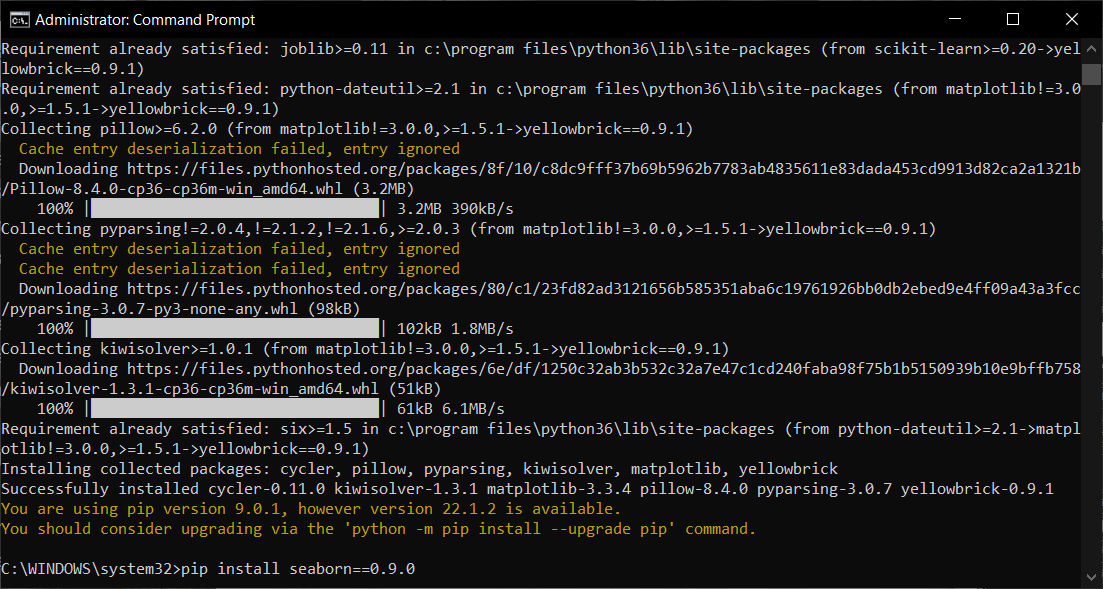
\includegraphics[width=0.7\linewidth, frame]{CA2-template/CM23.png}
       \caption{seaborn \label{fig:15}}
    \end{center}
\end{figure}

\item pip install matplotlib
\item pip install xgboost==0.81
\begin{figure}[H]
    \begin{center}
        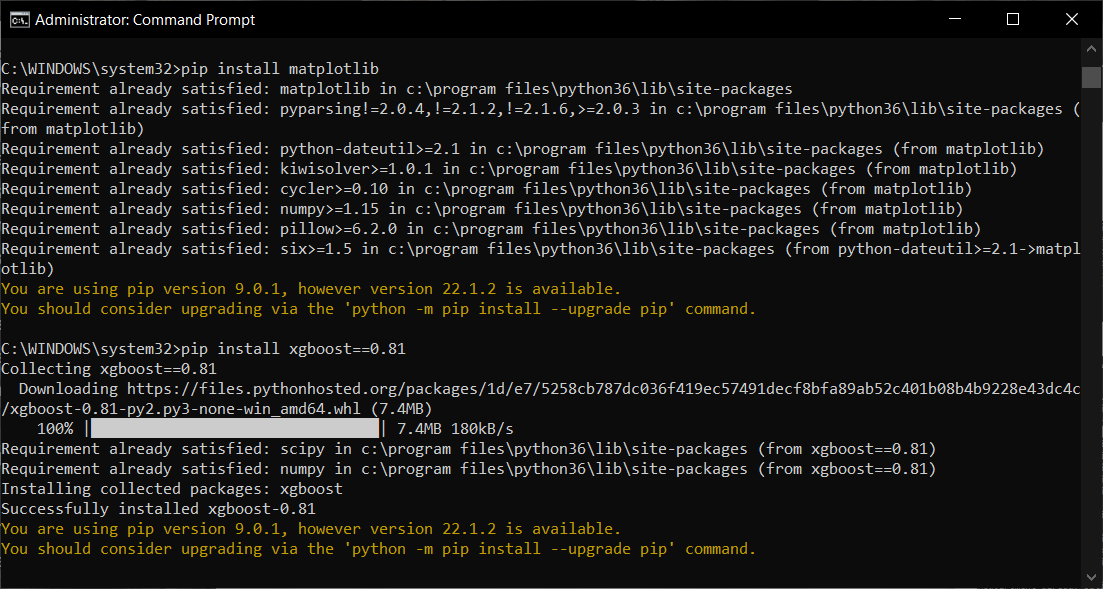
\includegraphics[width=0.7\linewidth, frame]{CA2-template/CM25.png}
       \caption{matplotlib and xgboost \label{fig:16}}
    \end{center}
\end{figure}

\item pip install mlxtend==0.14.0
\begin{figure}[H]
    \begin{center}
        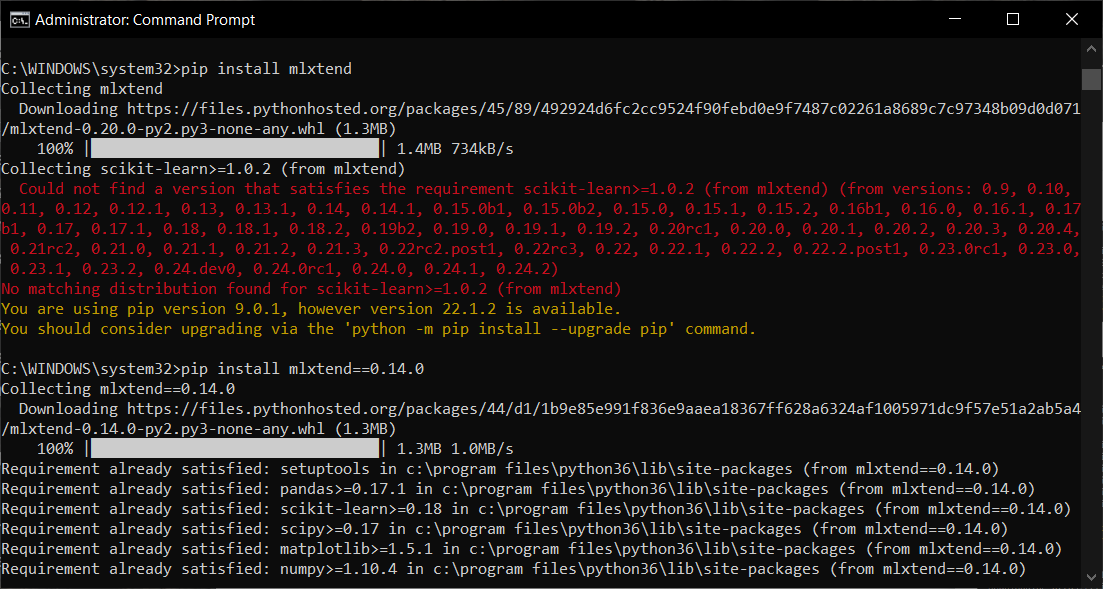
\includegraphics[width=0.7\linewidth, frame]{CA2-template/CM26.png}
       \caption{mlxtend \label{fig:17}}
    \end{center}
\end{figure}

\item pip install flask
\begin{figure}[H]
    \begin{center}
        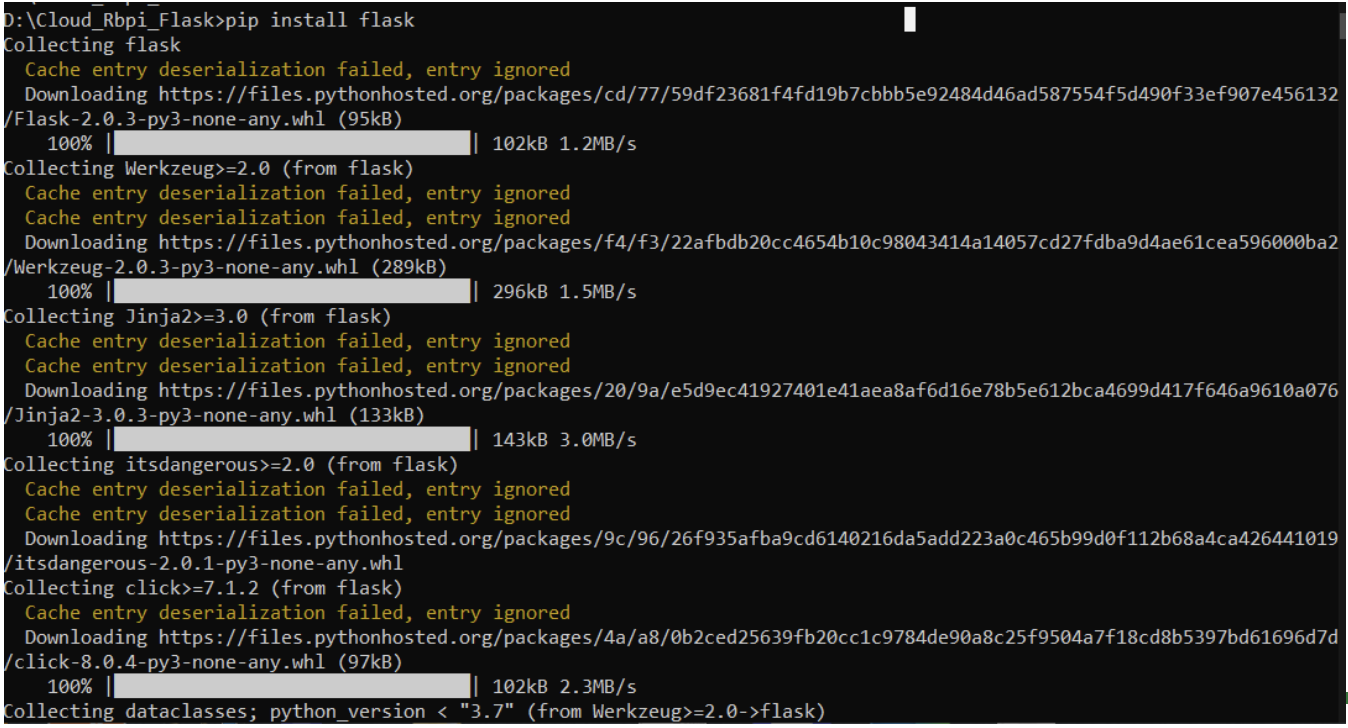
\includegraphics[width=0.7\linewidth, frame]{CA2-template/CM28.png}
       \caption{flask \label{fig:18}}
    \end{center}
\end{figure}
\end{itemize}

\subsubsection{Running the Application}
\begin{itemize}
    \item Connect to Raspberry Pi, and open Terminal. 
    \begin{figure}[H]
    \begin{center}
        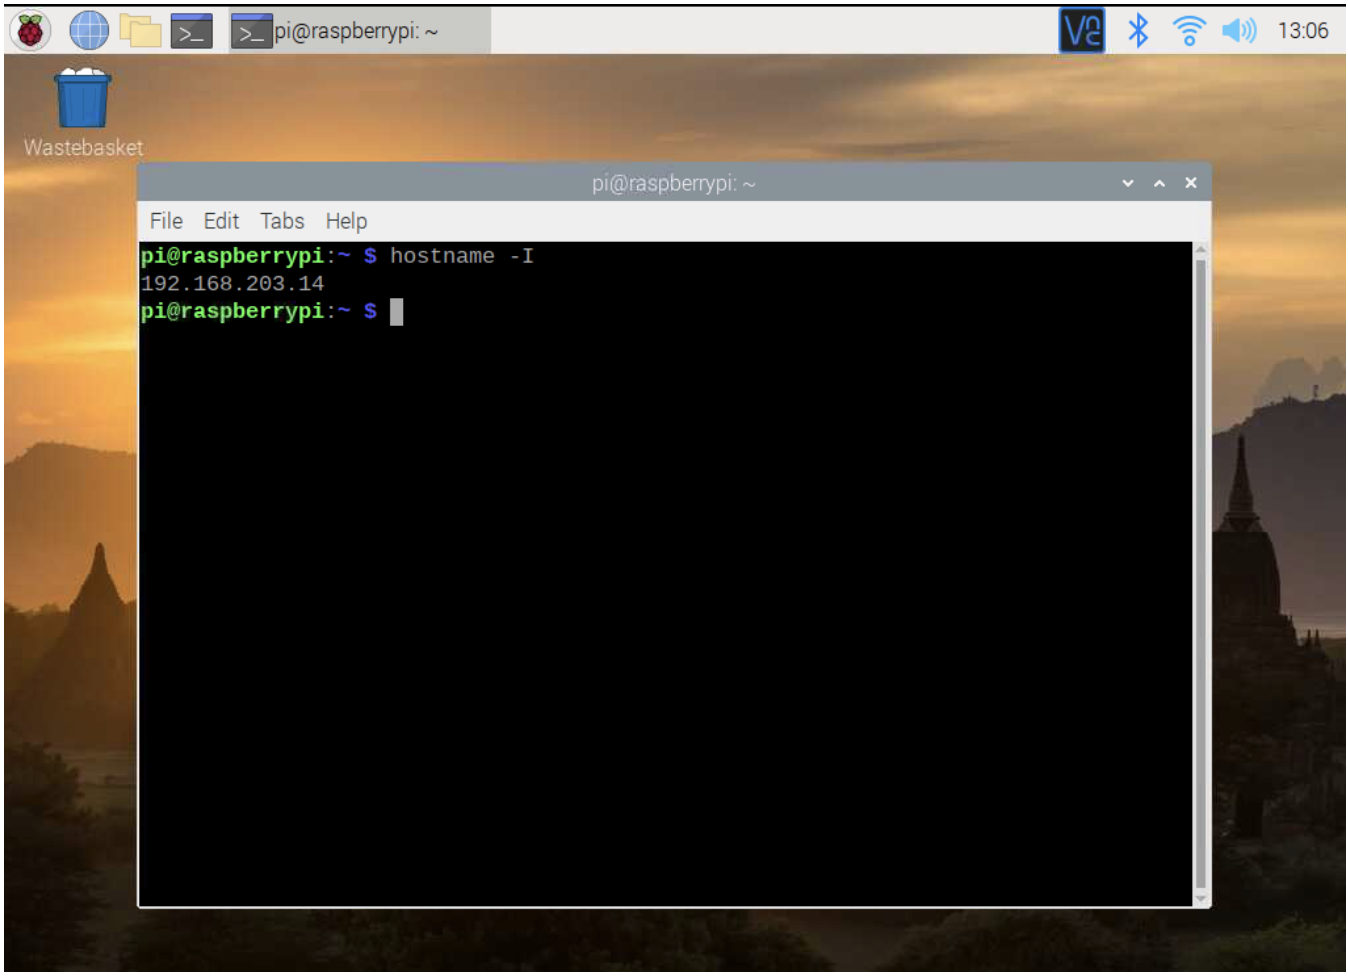
\includegraphics[width=0.7\linewidth, frame]{CA2-template/CM29.png}
       \caption{Raspberry Pi Terminal \label{fig:19}}
    \end{center}
\end{figure}

\item Check the IP address of Raspberry Pi using hostname -I command in the terminal
\begin{figure}[H]
    \begin{center}
        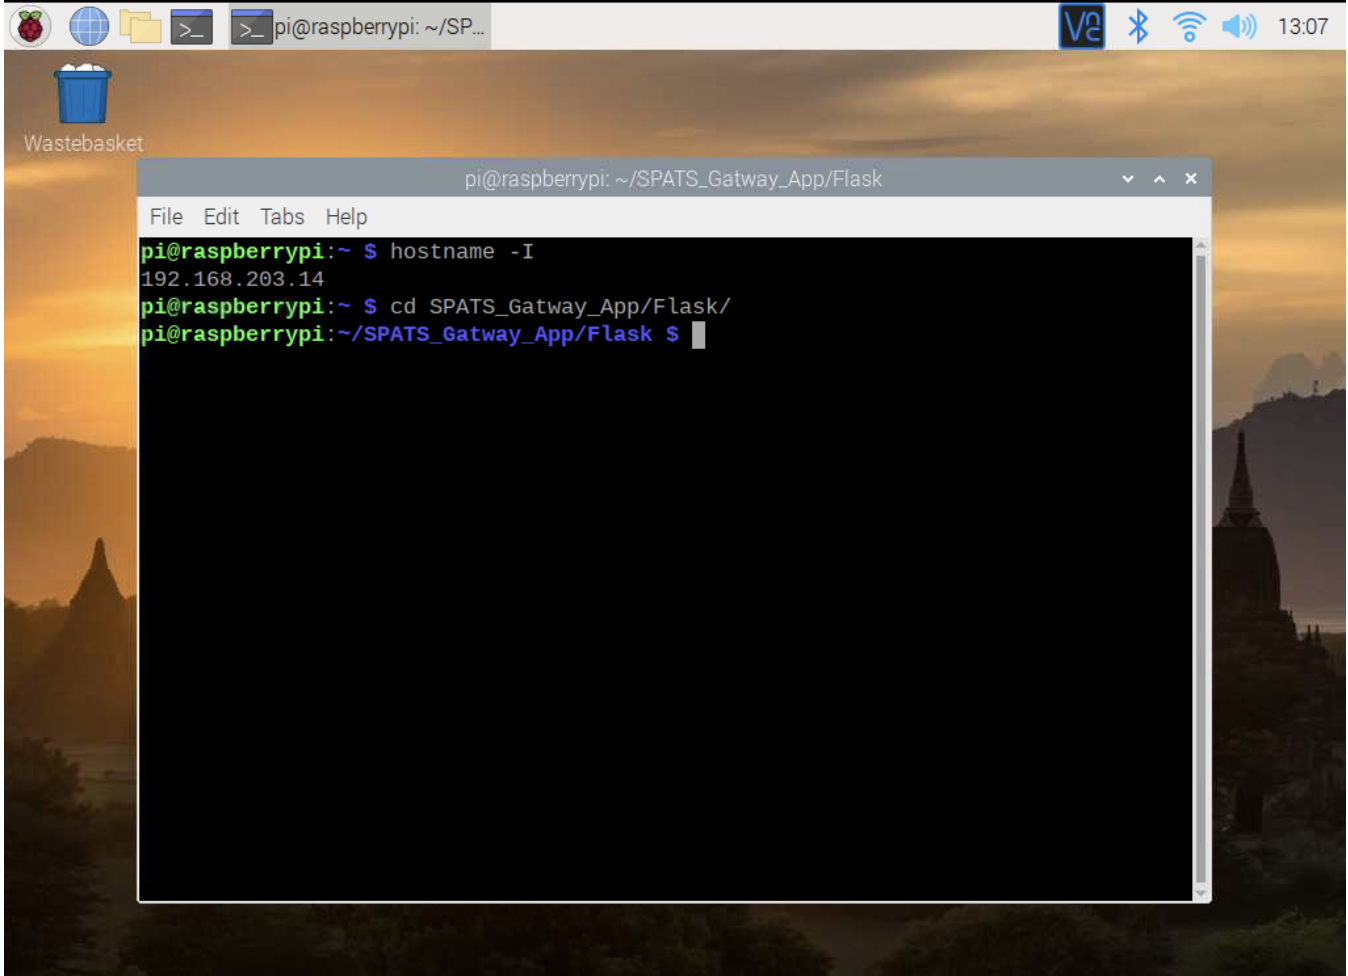
\includegraphics[width=0.7\linewidth, frame]{CA2-template/CM30.png}
       \caption{Check IP address \label{fig:20}}
    \end{center}
\end{figure}

\item Navigate to the application file and run app.py using python3 app.py command from the terminal
\begin{figure}[H]
    \begin{center}
        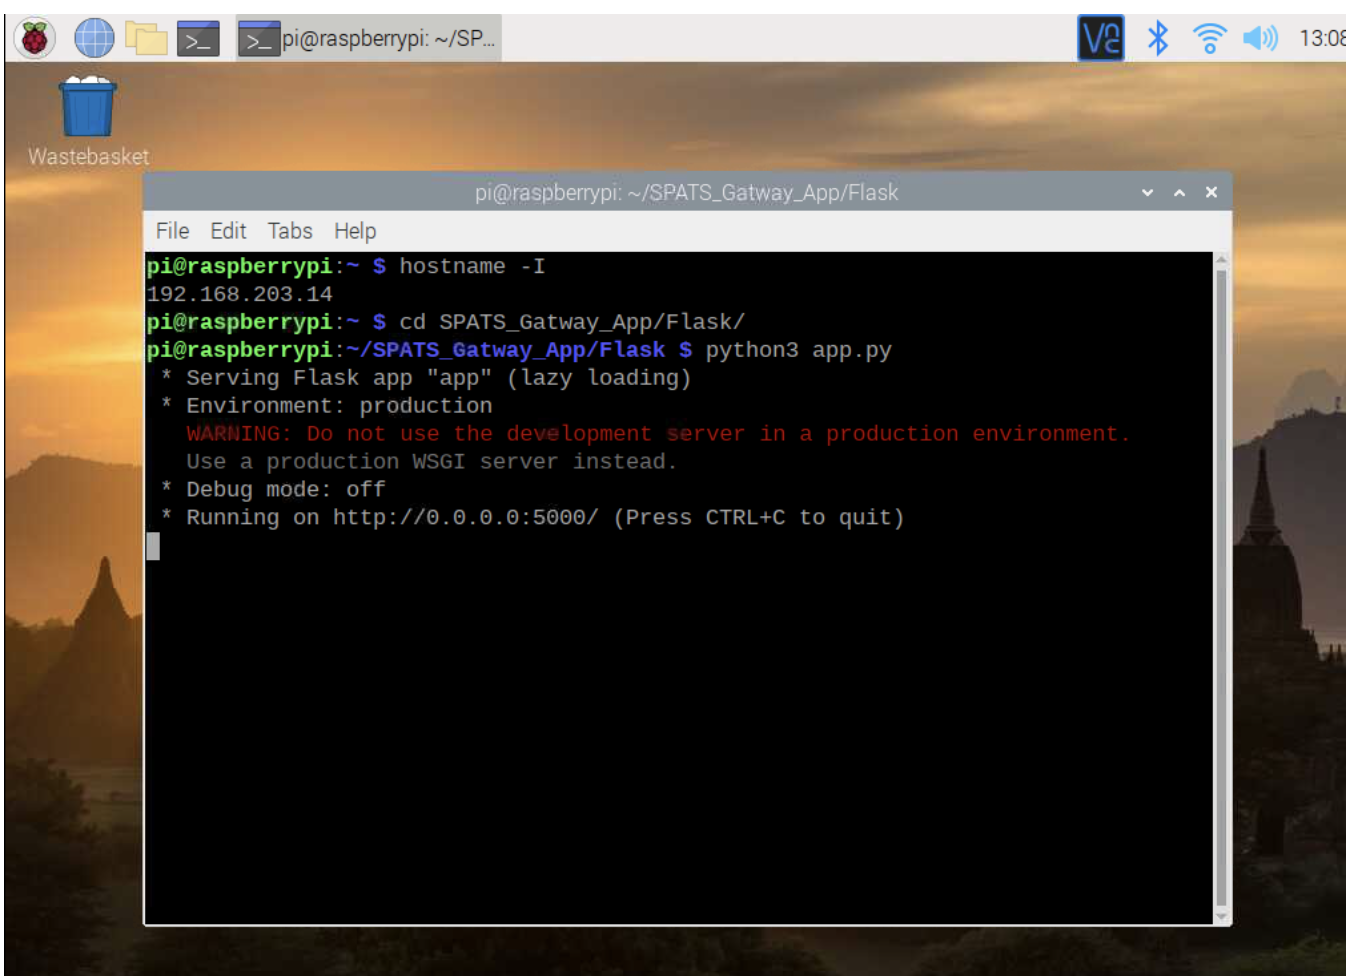
\includegraphics[width=0.7\linewidth, frame]{CA2-template/CM31.png}
       \caption{Run app.py \label{fig:21}}
    \end{center}
\end{figure}

\item The application is now running and can be accessed from any smart device connected within the same network. Enter 192.168.203.14:5000 in the browser URL to open the application as shown in the Figure \ref{fig:22}
\begin{figure}[H]
    \begin{center}
        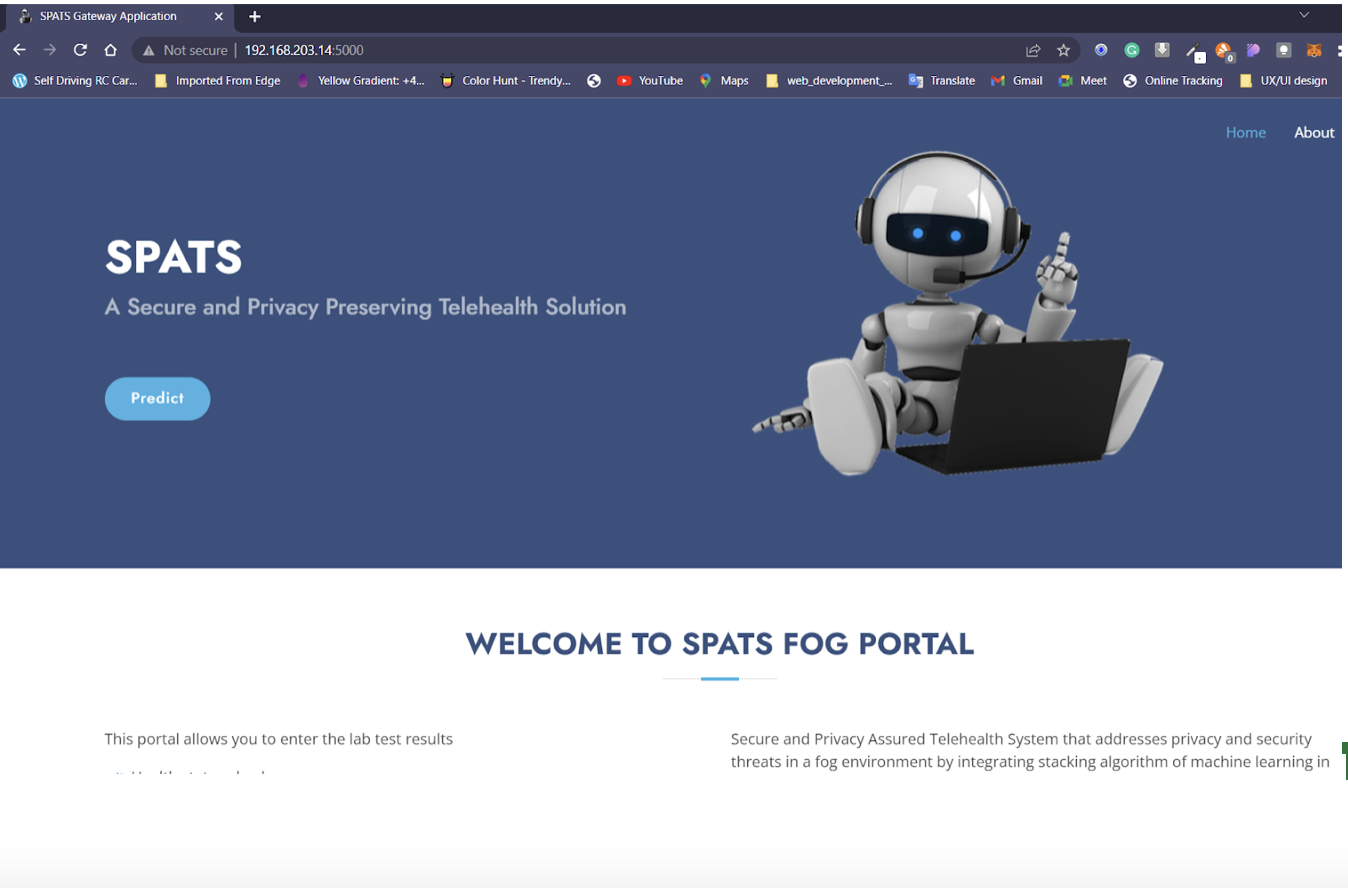
\includegraphics[width=0.7\linewidth, frame]{CA2-template/CM32.png}
       \caption{SPATS gateway application \label{fig:22}}
    \end{center}
\end{figure}

\end{itemize}

\section{Evaluation}
The efficiency of the SPATS system and the classifier used for training the models is evaluated using IFogSim tool and various performance measurement metrics in ML.

\subsection{Using IFogSim}
It is used to simulate and test the efficiency of the system when deployed in Cloud only mode versus Fog environment on the basis of Latency and Network usage.
\begin{itemize}
    \item Launch Eclipse IDE, Goto File menu and select "Open Project from Filesystem", navigate to the IFogSim folder and follow the on screen instructions.
    
    \item From Package explorer navigate and right click on org.fog.test.perfeval > New > Class to create a class in that package. 
    \begin{figure}[H]
    \begin{center}
        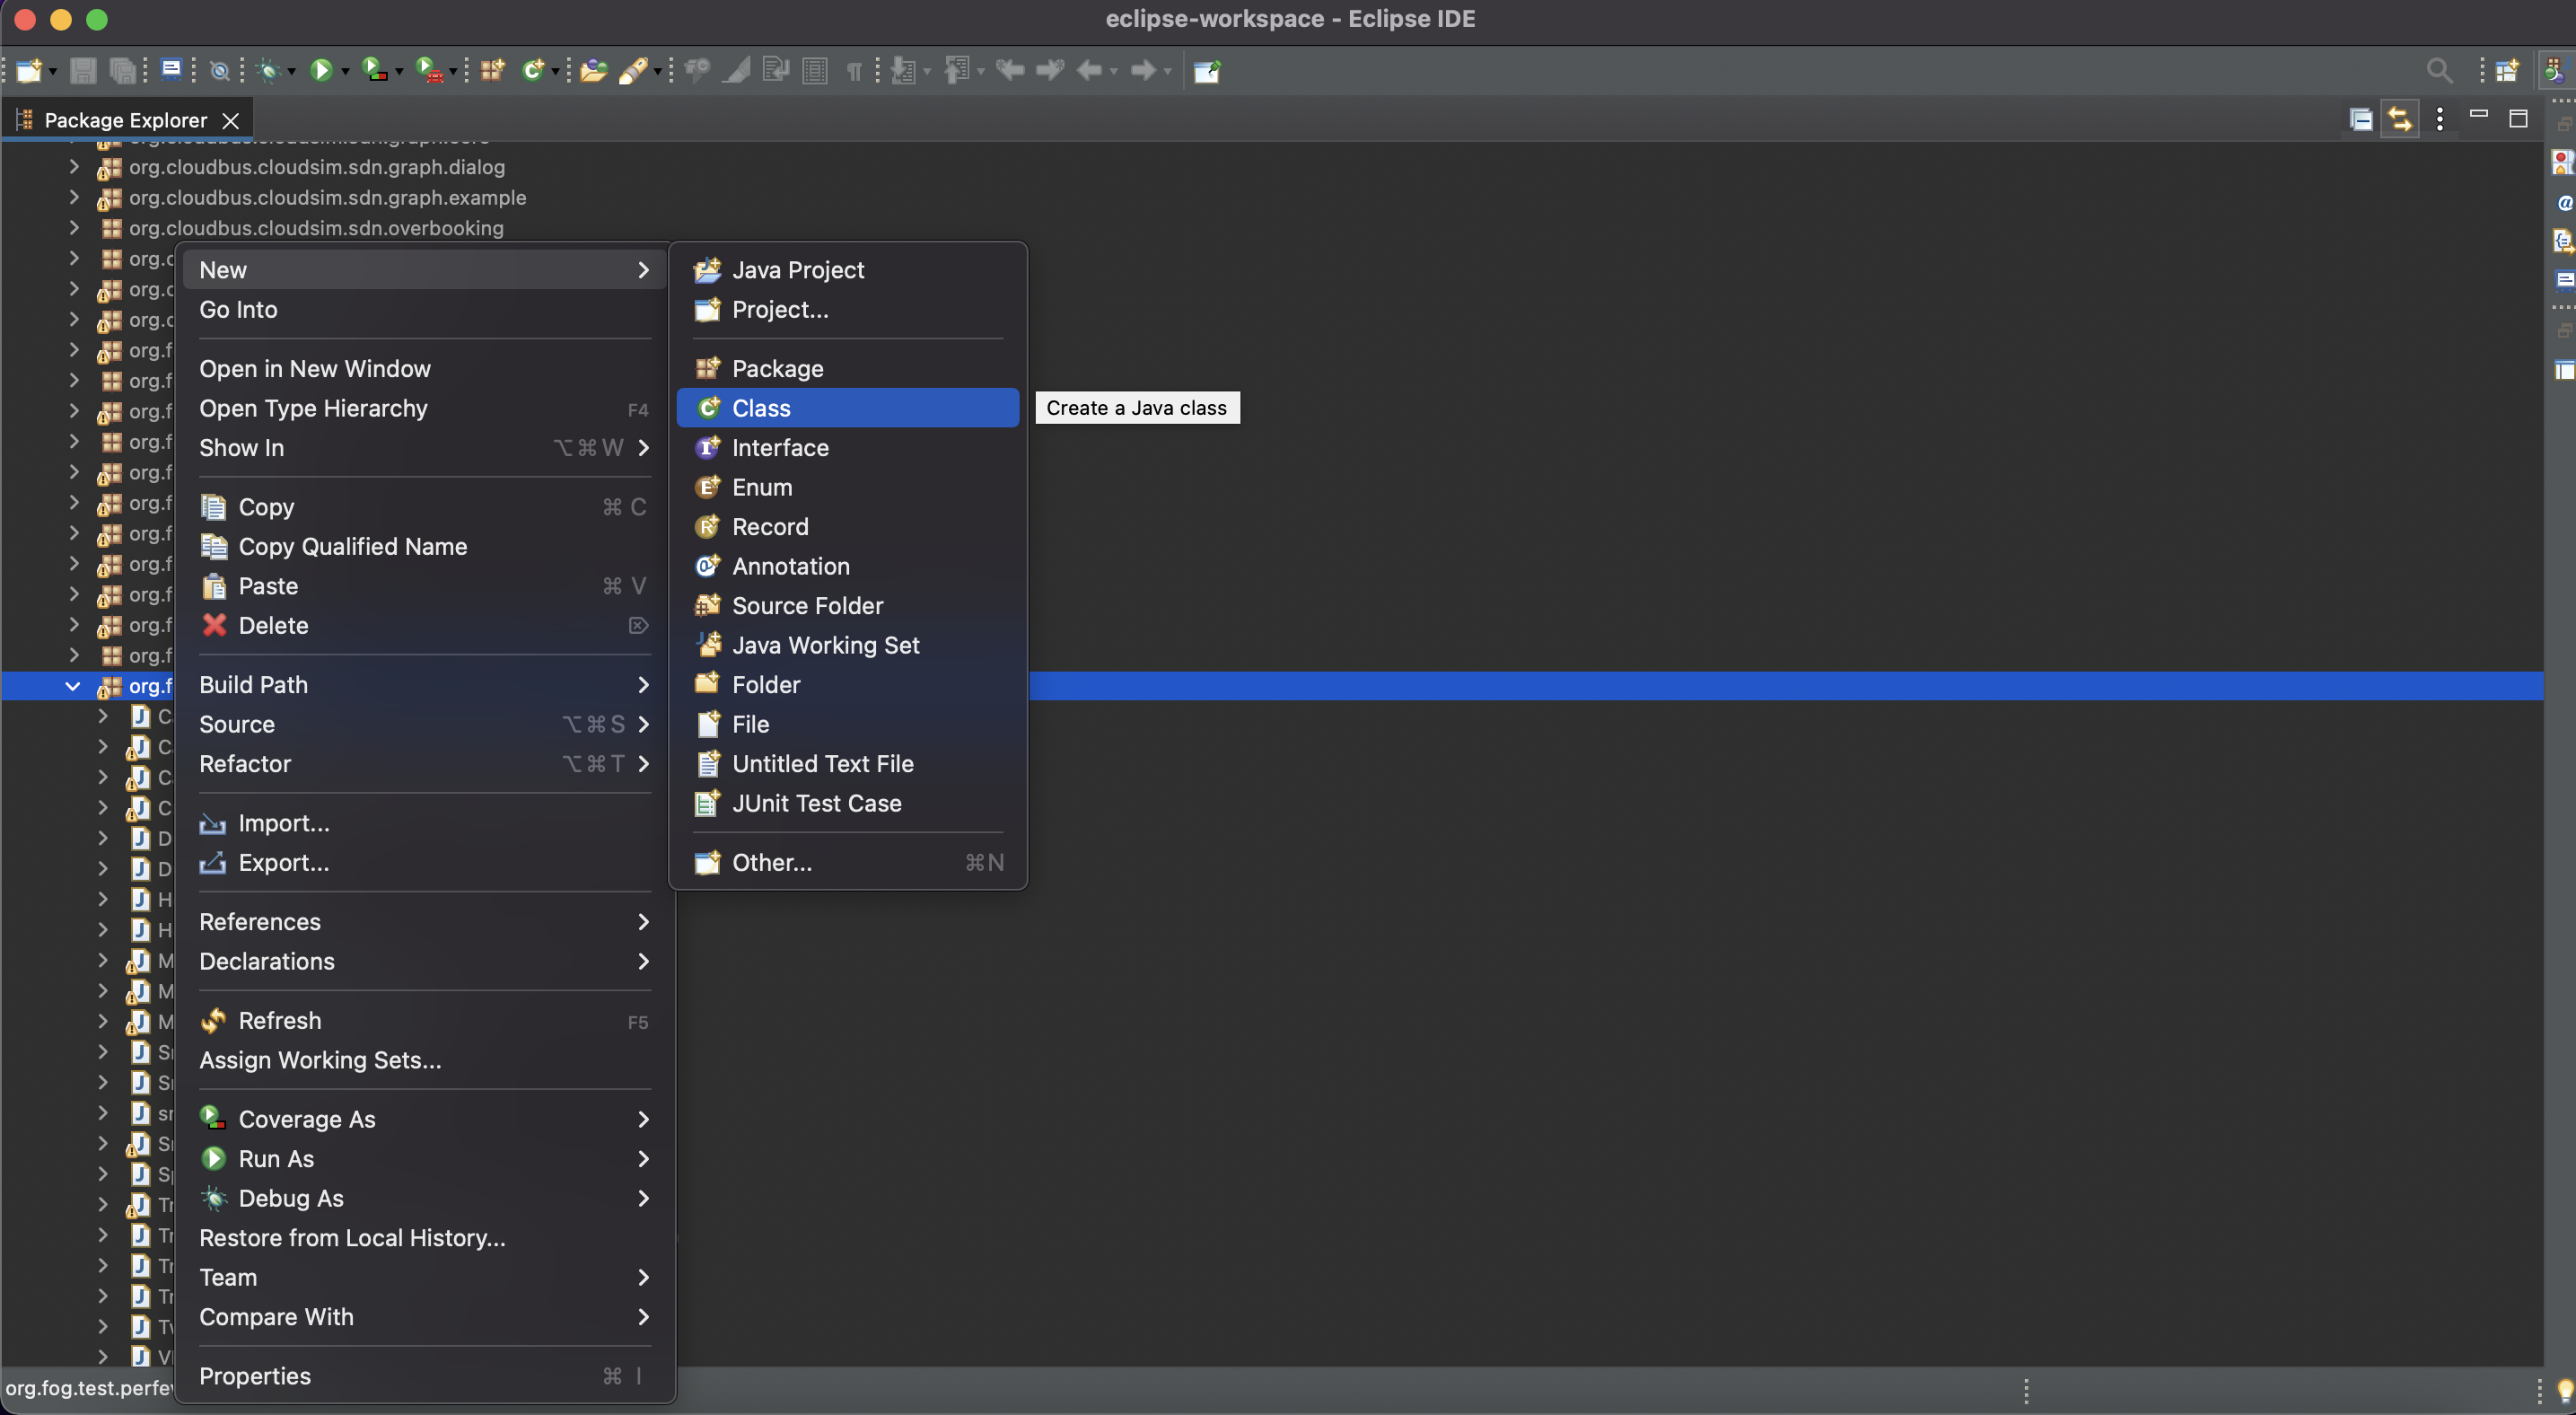
\includegraphics[width=0.7\linewidth, frame]{CA2-template/CM33.png}
       \caption{Eclipse IDE \label{fig:23}}
    \end{center}
\end{figure}

\item Give Spats\_Sim as the name of the class and Finish
\begin{figure}[H]
    \begin{center}
        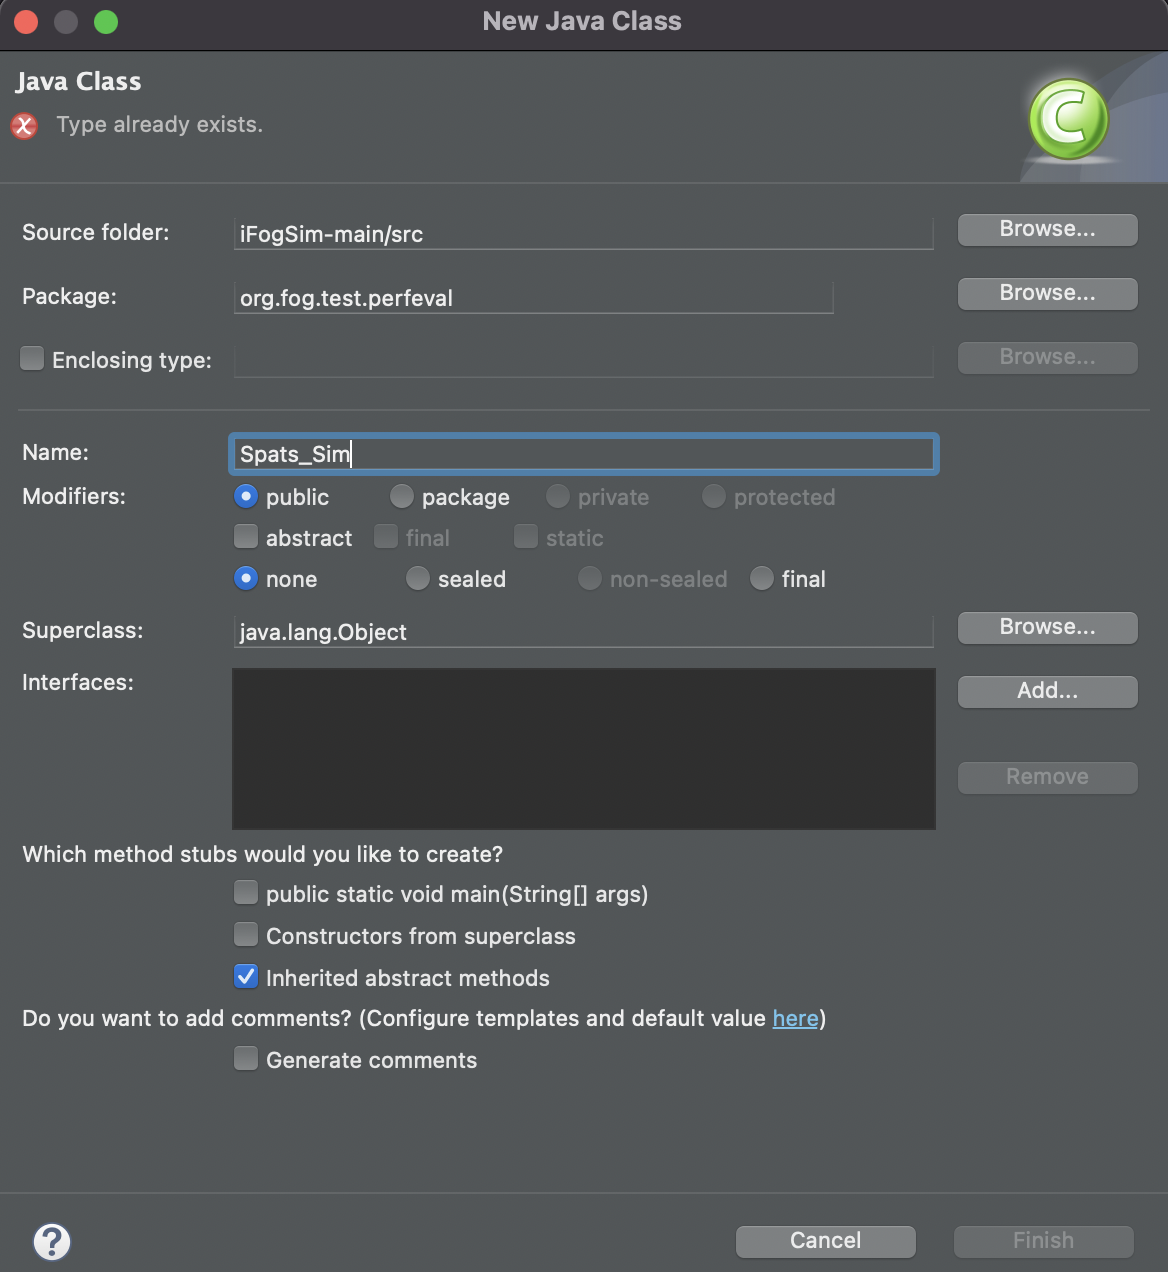
\includegraphics[width=0.7\linewidth, frame]{CA2-template/CM34.png}
       \caption{Create New Class \label{fig:24}}
    \end{center}
\end{figure}

\item Copy paste the contents of Spats\_sim.java fail to this file 
\begin{figure}[H]
    \begin{center}
        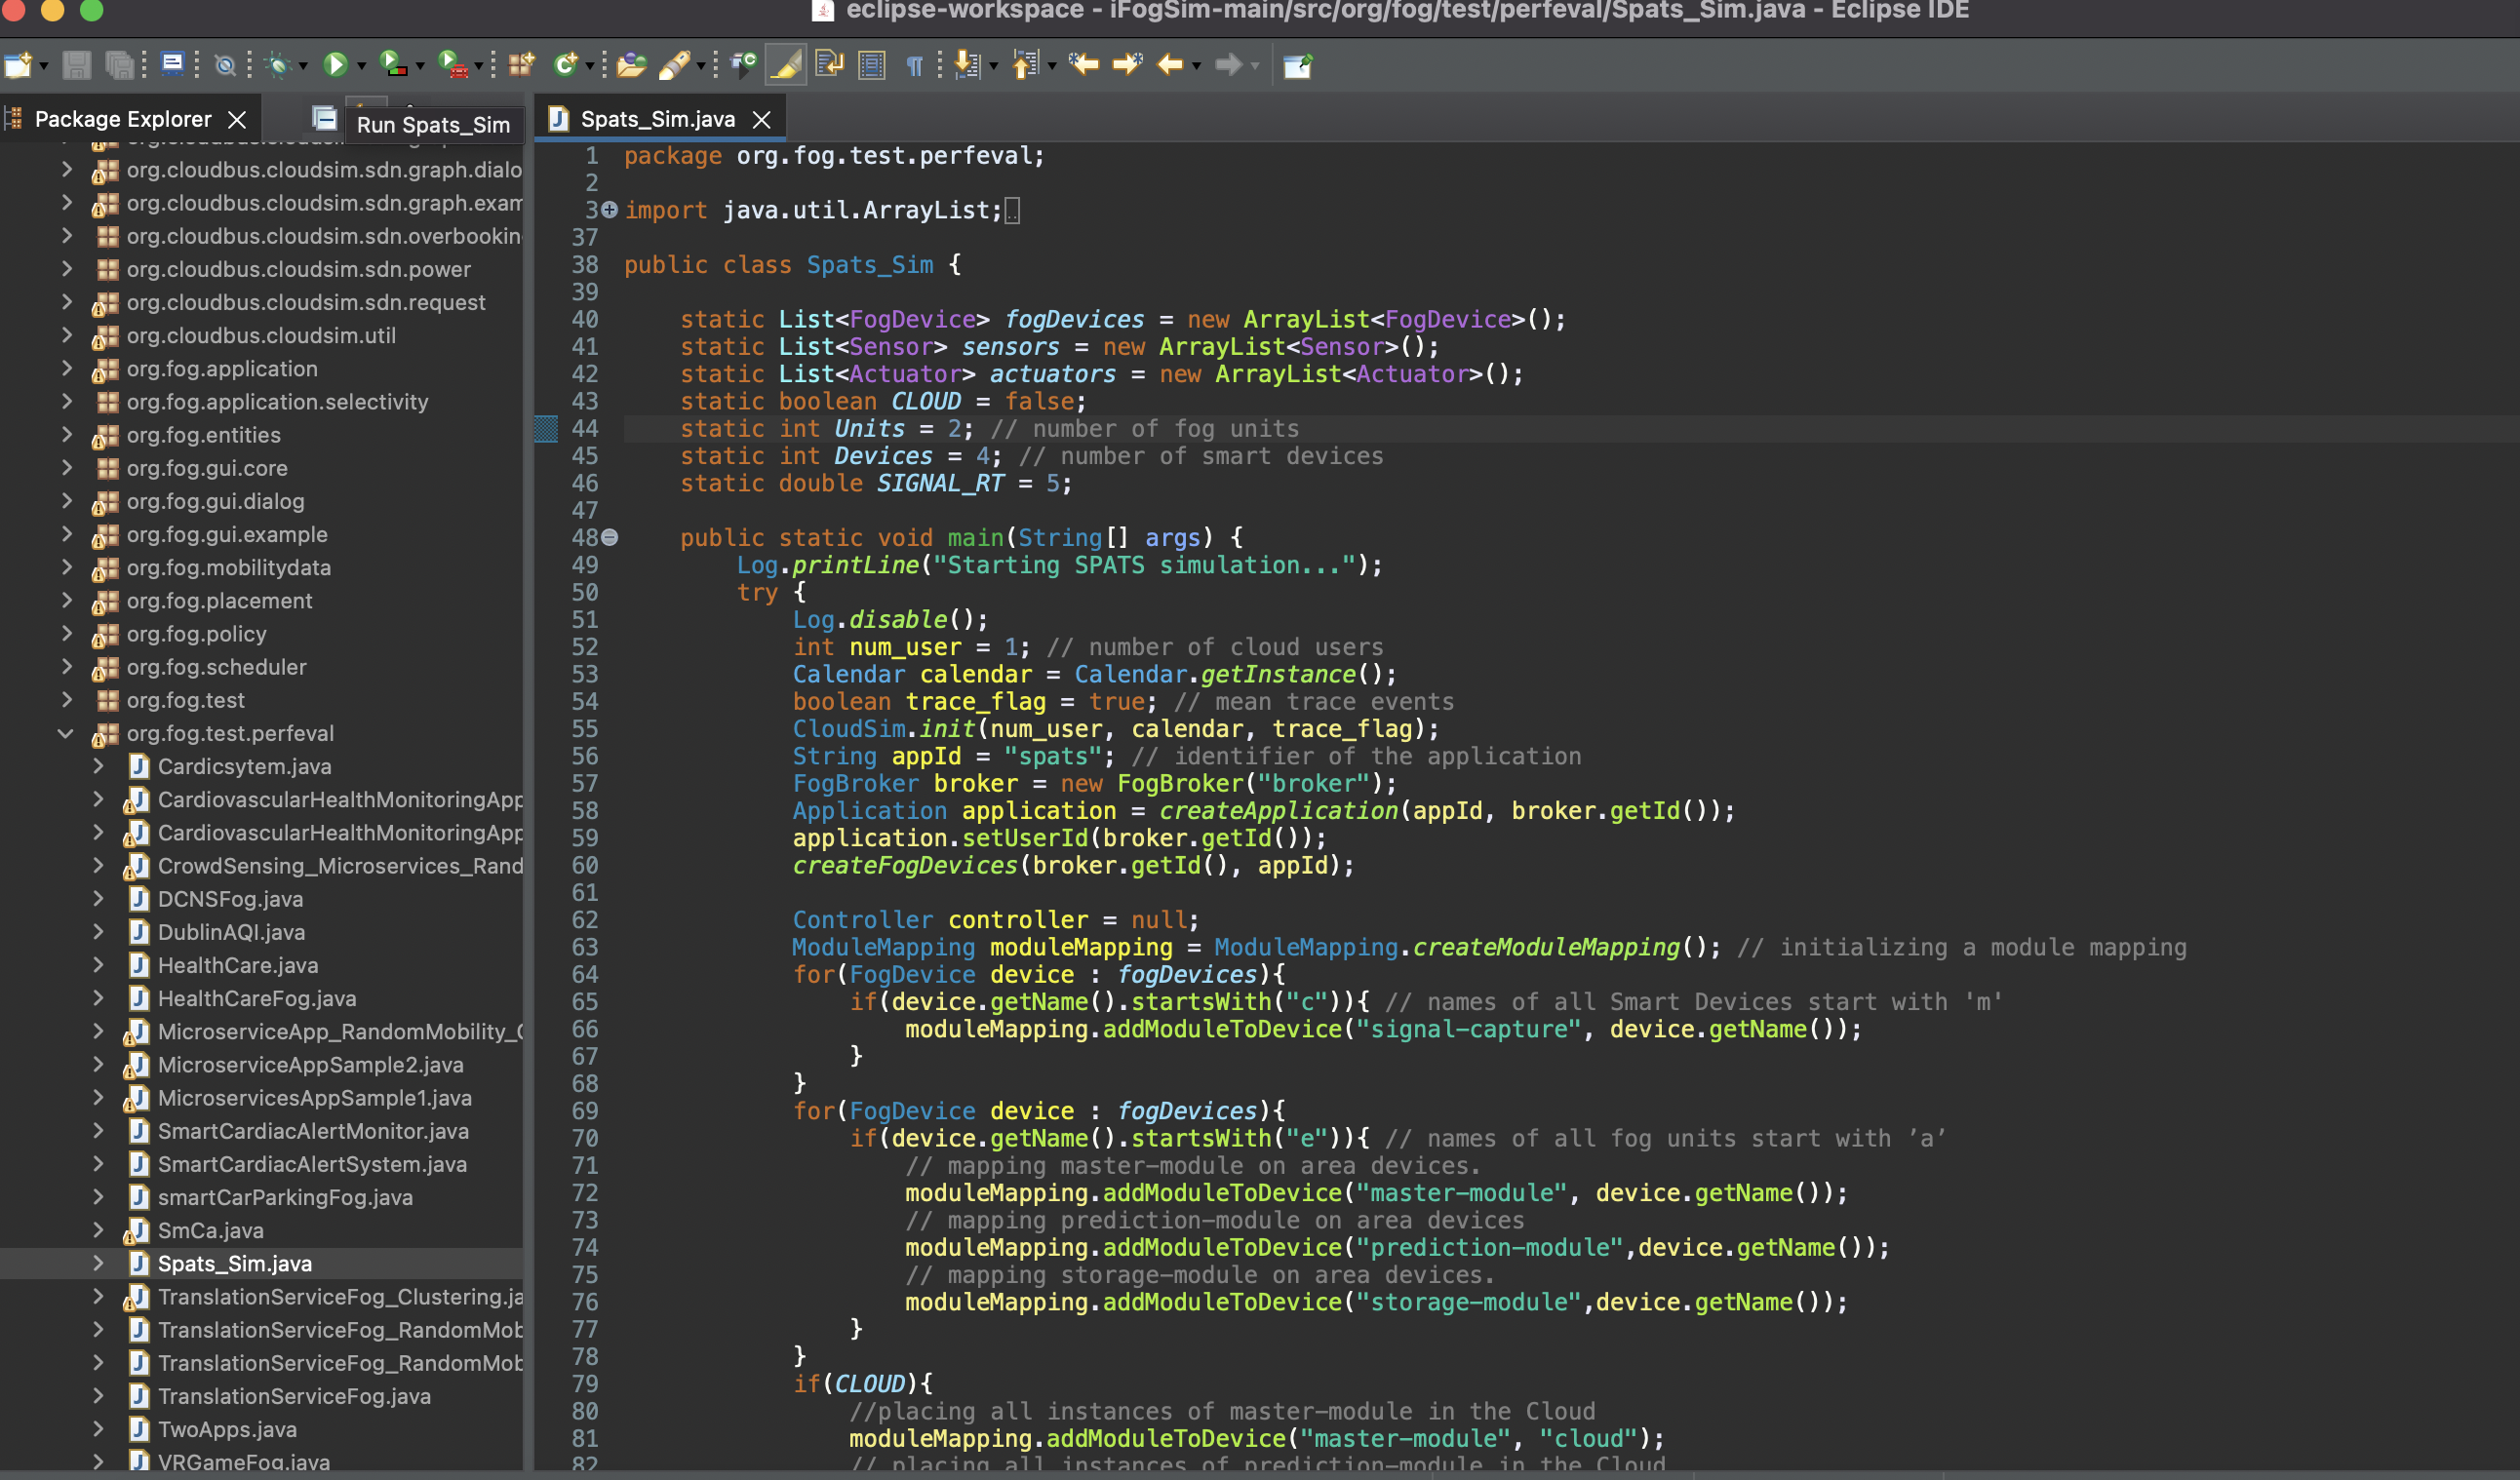
\includegraphics[width=0.7\linewidth, frame]{CA2-template/CM35.png}
       \caption{Spats_sim code \label{fig:25}}
    \end{center}
\end{figure}

\item Click the green play button on top to run the code. Change the values in the highlighted section to simulate based on different scenarios as shown in Fig \ref{fig:26} and Fig \ref{fig:27}
\begin{figure}[H]
    \begin{center}
        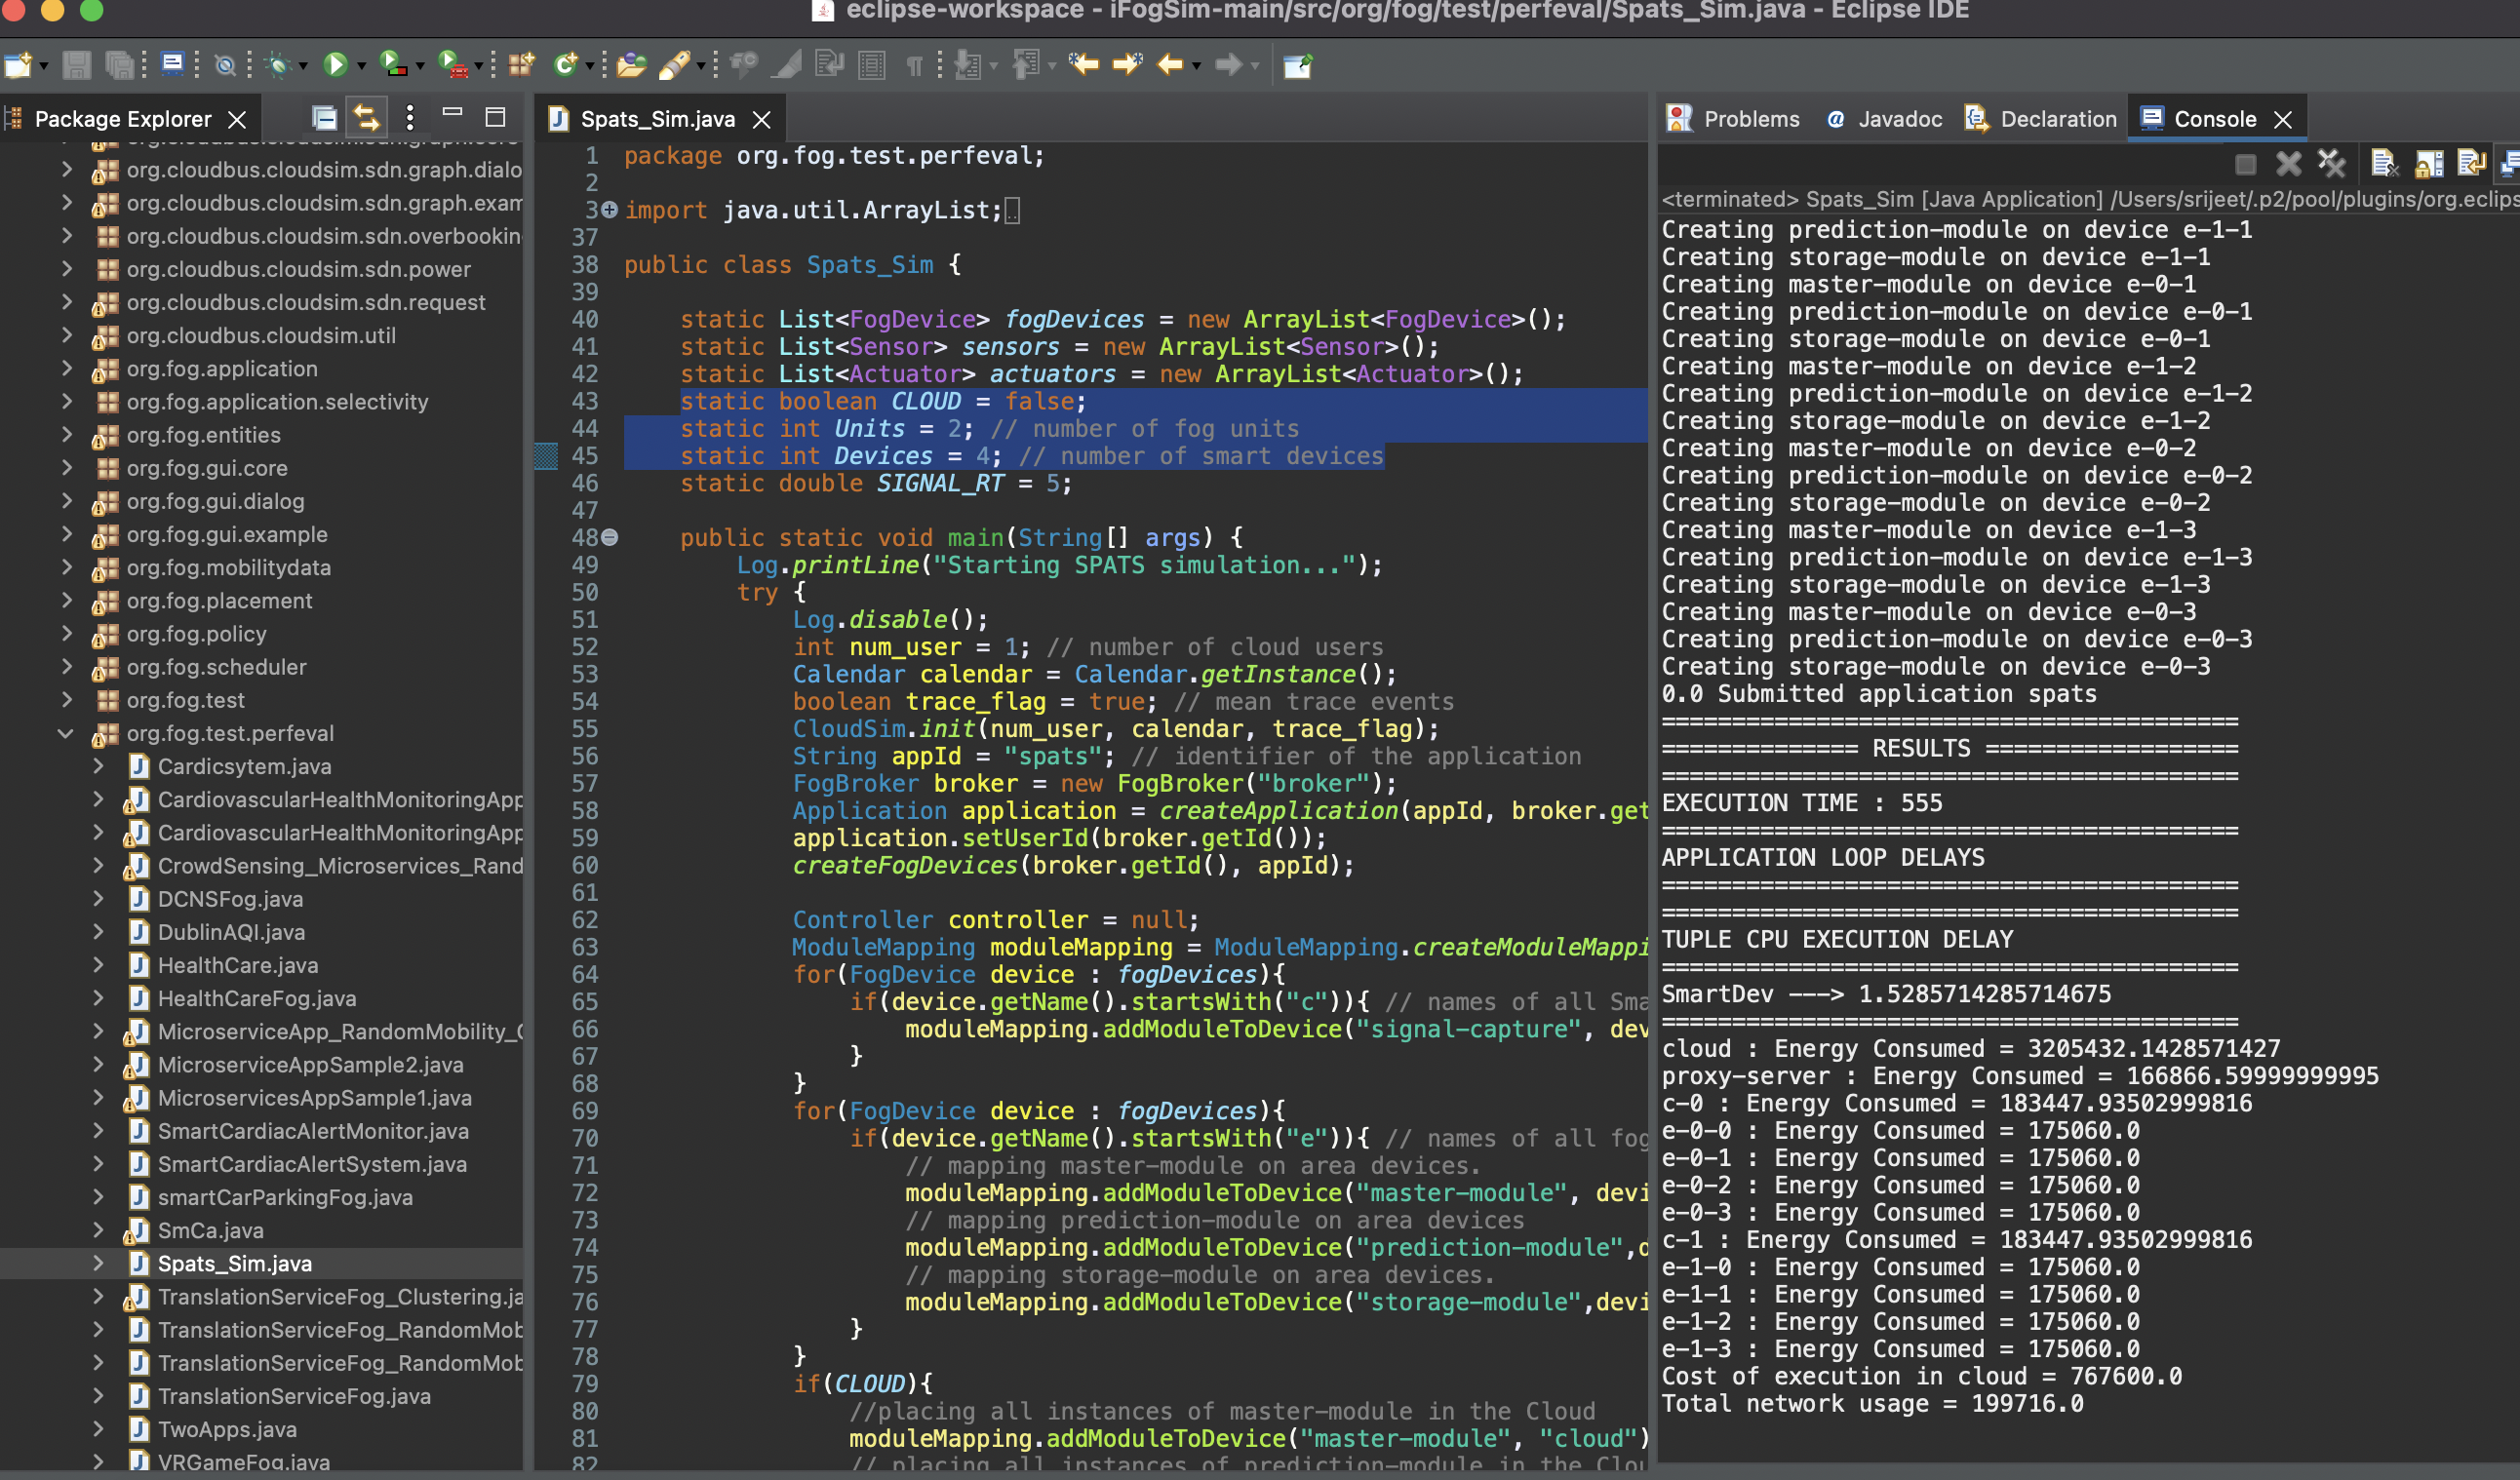
\includegraphics[width=0.7\linewidth, frame]{CA2-template/CM36.png}
       \caption{Run the code (in Fog environment) \label{fig:26}}
    \end{center}
\end{figure}

\begin{figure}[H]
    \begin{center}
        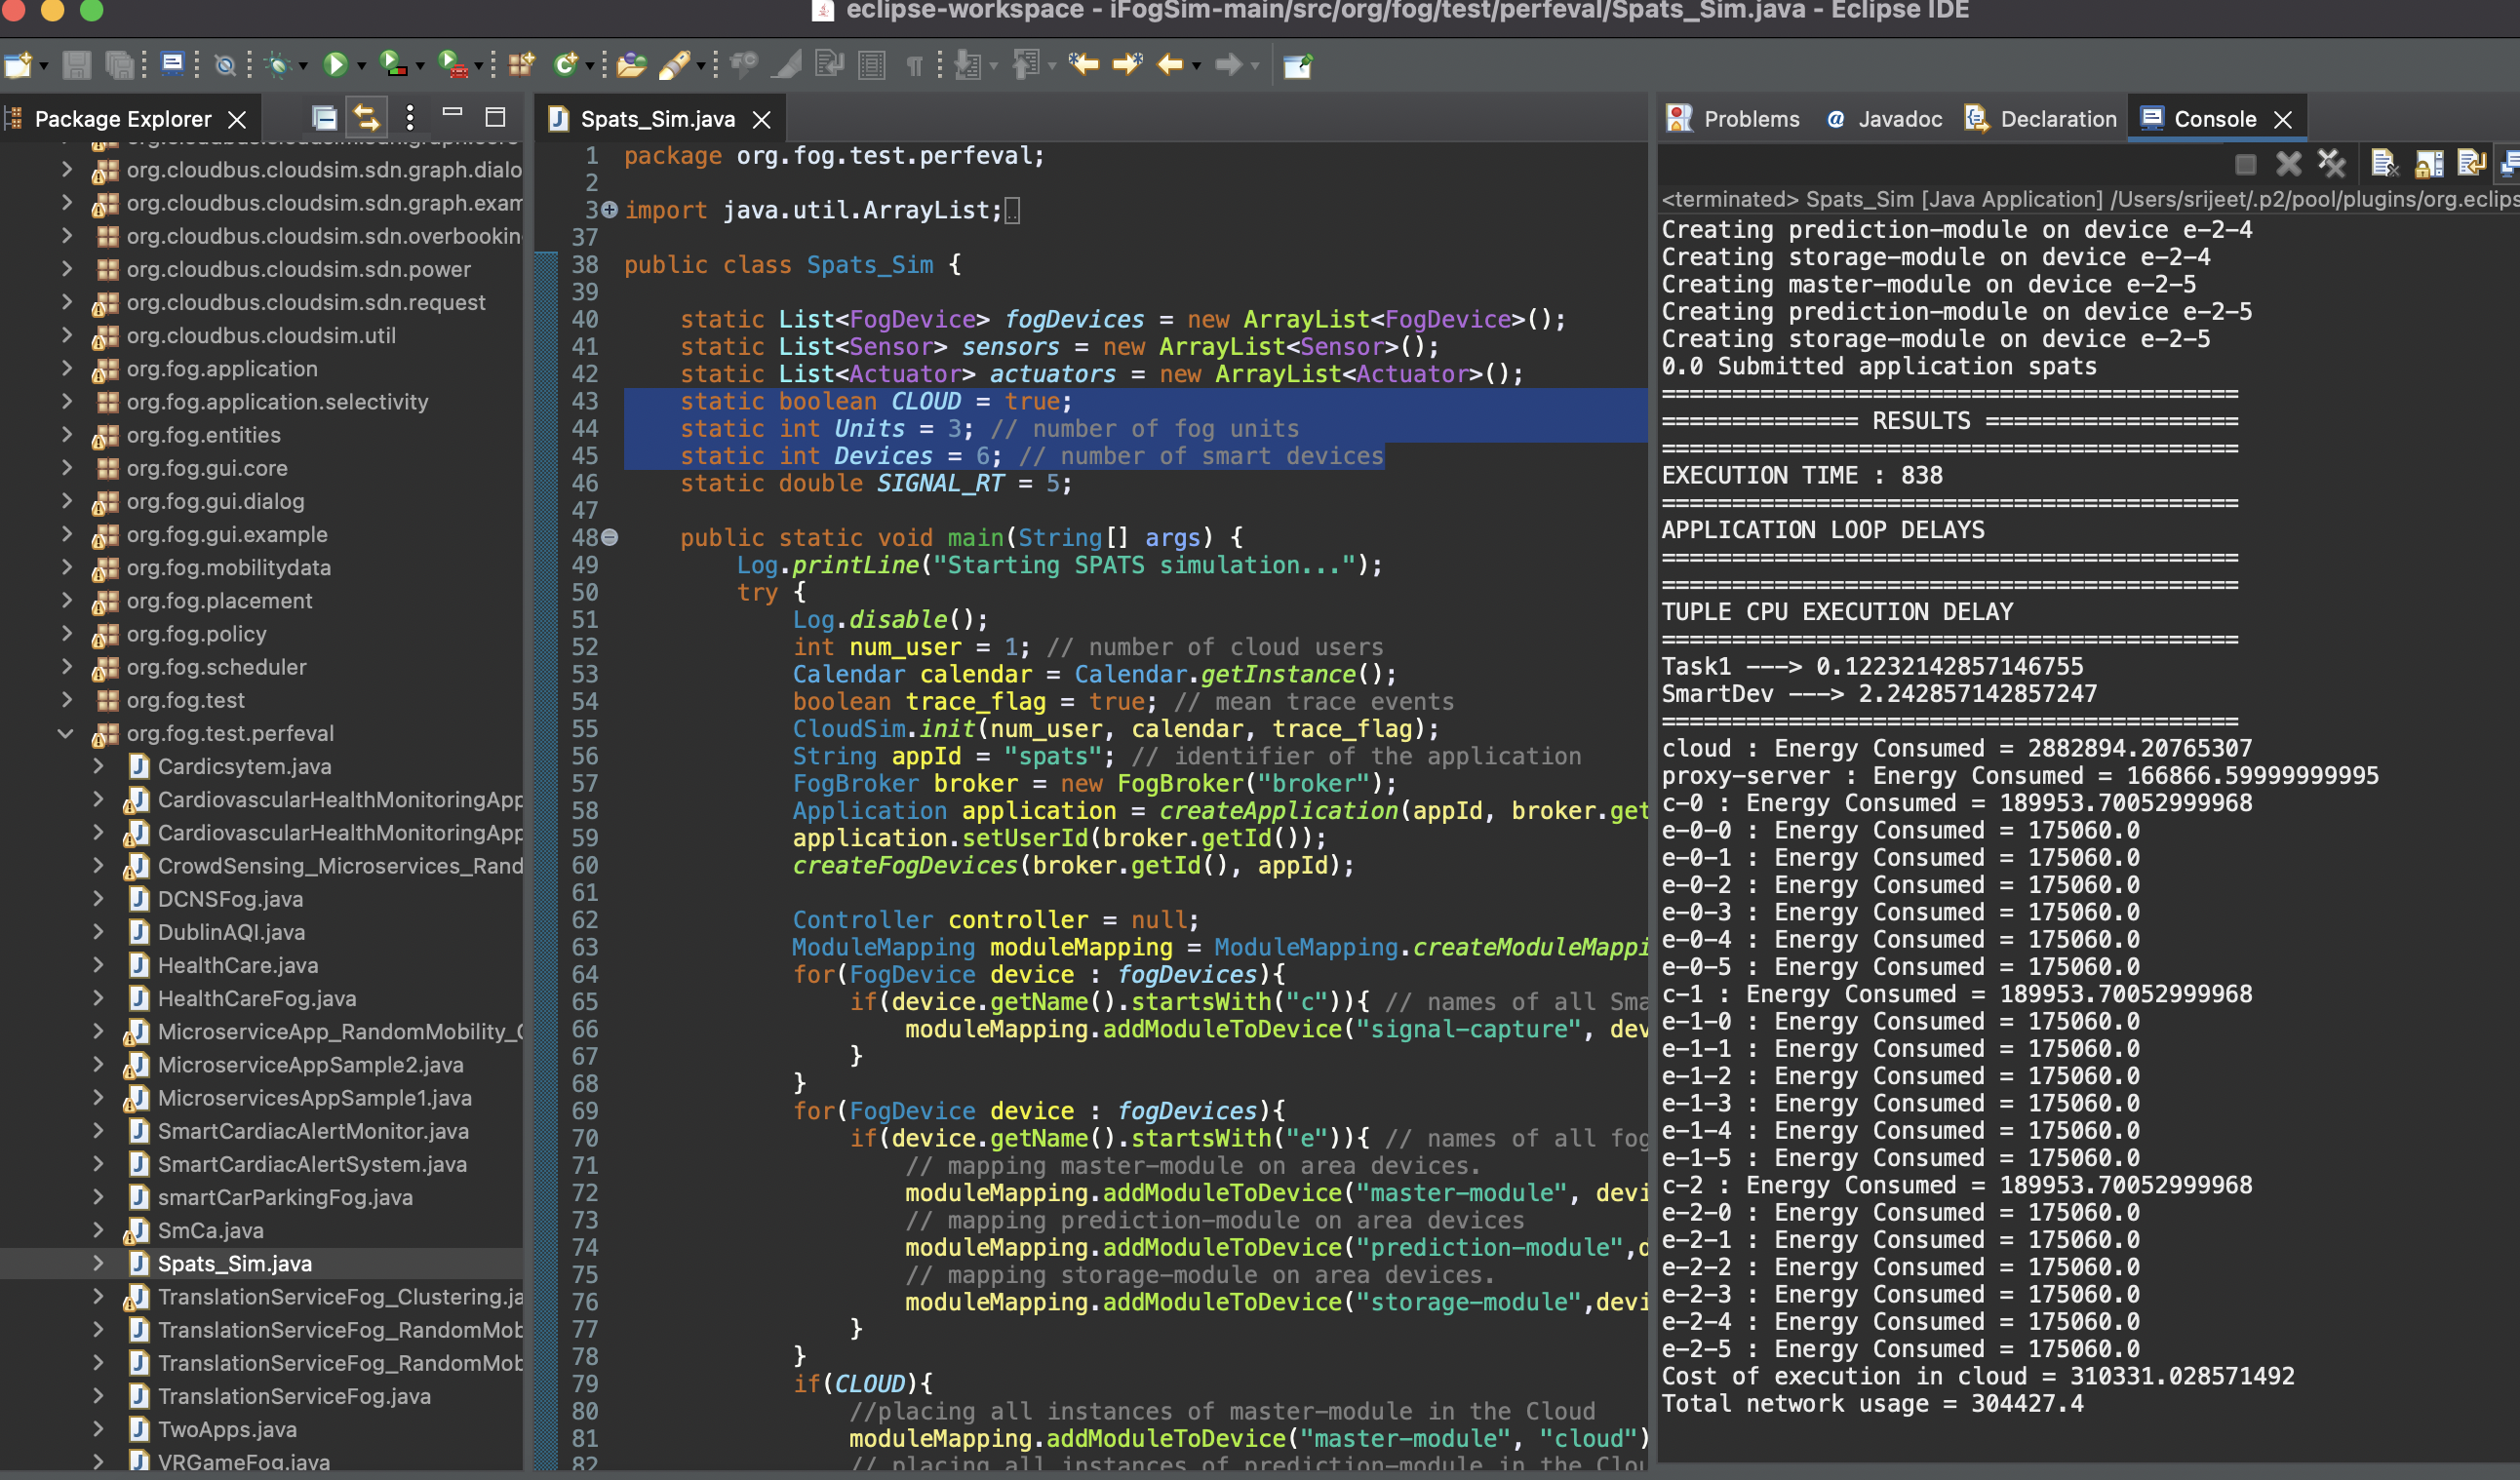
\includegraphics[width=0.7\linewidth, frame]{CA2-template/CM37.png}
       \caption{Run the code (in cloud environment) \label{fig:27}}
    \end{center}
\end{figure}
\end{itemize}

\subsection{Performance of Classifier}
\begin{itemize}
    \item Launch VS code IDE 
    \begin{figure}[H]
    \begin{center}
        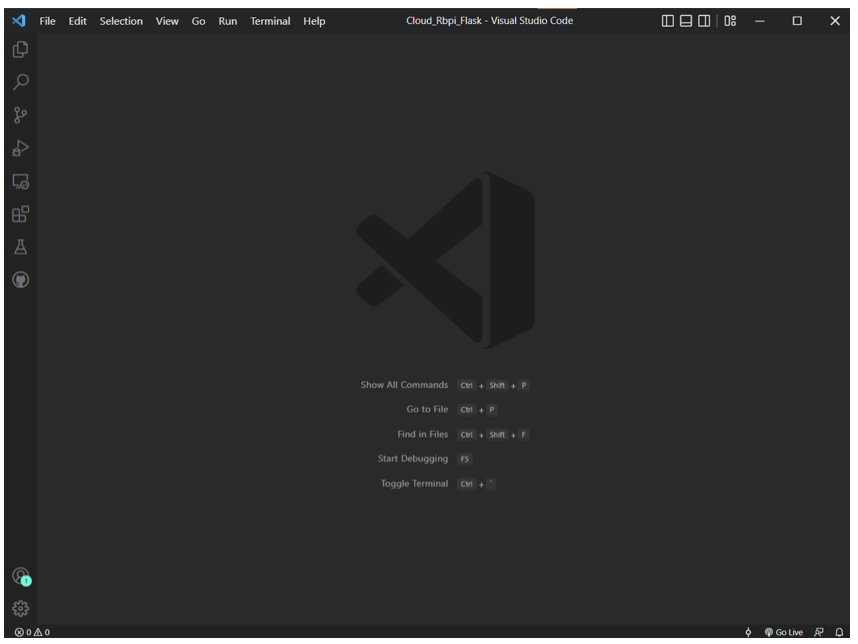
\includegraphics[width=0.7\linewidth, frame]{CA2-template/CM38.png}
       \caption{VS Code IDE \label{fig:28}}
    \end{center}
\end{figure}

\item Select Open Folder from File menu and navigate to the gateway application folder and click Open
\begin{figure}[H]
    \begin{center}
        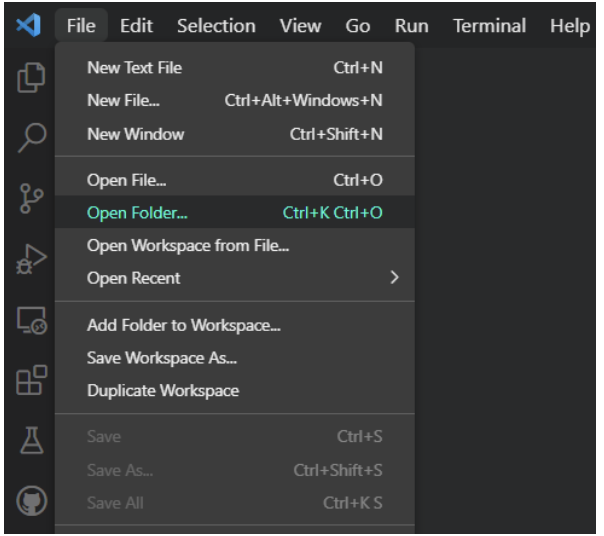
\includegraphics[width=0.7\linewidth, frame]{CA2-template/CM39.png}
       \caption{Open Folder \label{fig:29}}
    \end{center}
\end{figure}

\item From Explorer pane select algo.py
\begin{figure}[H]
    \begin{center}
        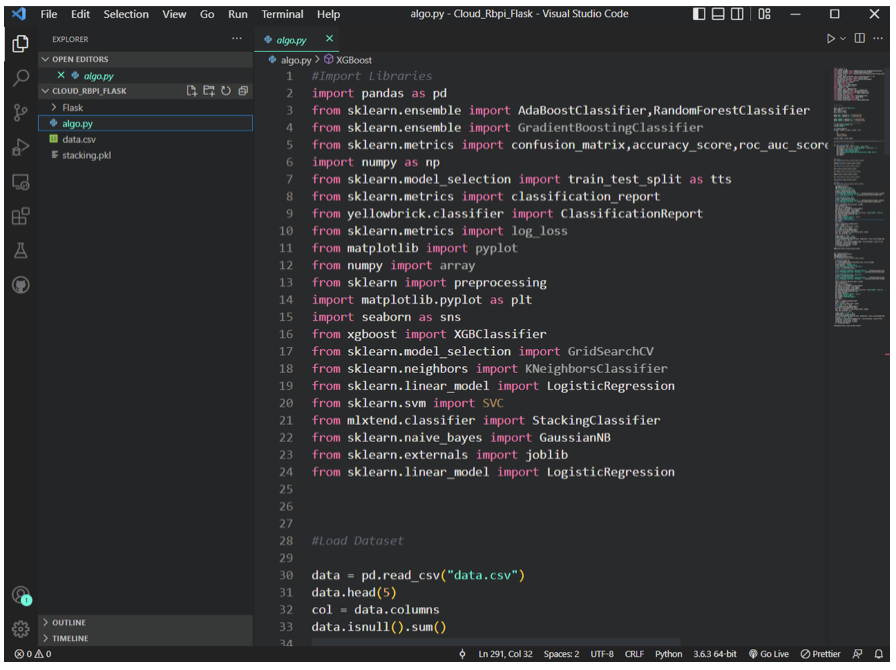
\includegraphics[width=0.7\linewidth, frame]{CA2-template/CM40.png}
       \caption{algo.py \label{fig:30}}
    \end{center}
\end{figure}

\item Click on the play button on top right corner of the window pane to run the code. It will keep showing the performance efficiency of different classifiers in terms of there Confusion graph, ROC graph, Accuracy, Precision and F1 Score as shown in Fig \ref{fig:31}
\begin{figure}[H]
    \begin{center}
        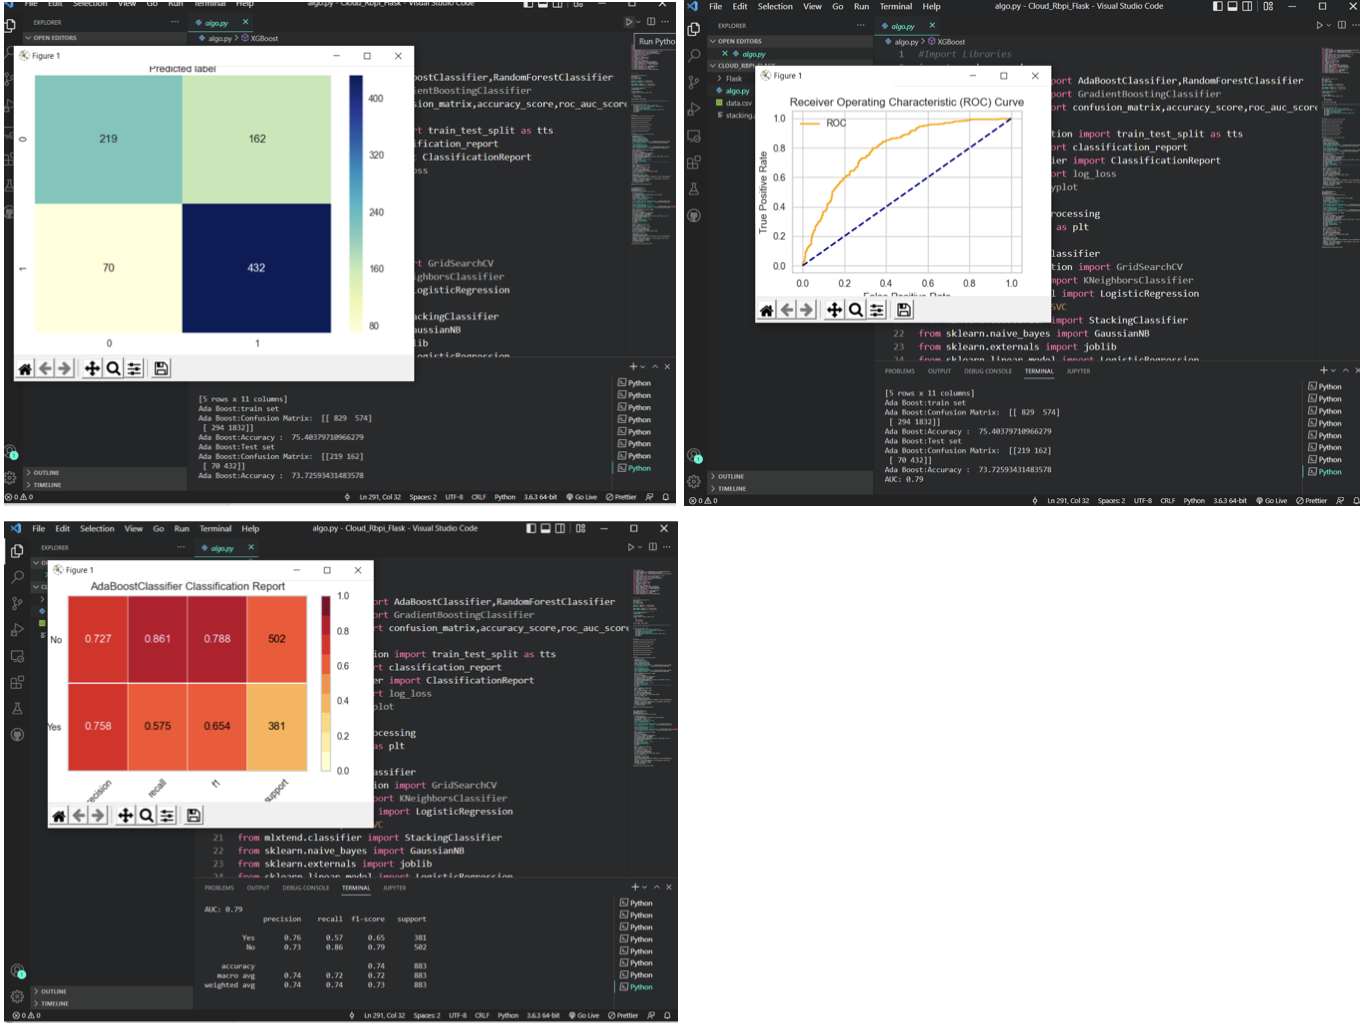
\includegraphics[width=0.7\linewidth, frame]{CA2-template/CM41.png}
       \caption{Code run - Output \label{fig:31}}
    \end{center}
\end{figure}
    
\end{itemize}

\begin{thebibliography}{40}

\bibitem{1} R. P. Ltd, “Raspberry Pi 4 Model B specifications,” Raspberry Pi. https://www.raspberrypi.com/products/raspberry-pi-4-model-b/.

\bibitem{2} “Download Visual Studio Tools - Install Free for Windows, Mac, Linux,” Visual Studio. https://visualstudio.microsoft.com/downloads/.

\bibitem{3} “Install Visual Studio | Microsoft Docs.” https://docs.microsoft.com/en-us/visualstudio/install/install-visual-studio?view=vs-2022.

\bibitem{4} “Using Python on Windows — Python 3.10.6 documentation.” https://docs.python.org/3/using/windows.html.

\bibitem{5} “Eclipse Installer 2022-06 R | Eclipse Packages.” https://www.eclipse.org/downloads/packages/installer.

\bibitem{6} “iFogSim2 (The New Version).” The Cloud Computing and Distributed Systems (CLOUDS) Laboratory, Jul. 10, 2022. Available: https://github.com/Cloudslab/iFogSim


\end{thebibliography}

\end{document}